\documentclass[conference]{IEEEtran}
\IEEEoverridecommandlockouts

\usepackage{graphicx}
\usepackage{amsmath,amssymb,amsfonts,amsthm}
\DeclareMathOperator{\lcm}{lcm}
\usepackage{paralist}
\usepackage{color}
\usepackage[hidelinks]{hyperref}
\usepackage{xspace}
\usepackage{algorithm}
\usepackage{algorithmicx}
\usepackage{todonotes}
\usepackage{verbatim}

\usepackage{array}
\newcolumntype{L}[1]{>{\raggedright\let\newline\\\arraybackslash\hspace{0pt}}m{#1}}
\newcolumntype{C}[1]{>{\centering\let\newline\\\arraybackslash\hspace{0pt}}m{#1}}
\newcolumntype{R}[1]{>{\raggedleft\let\newline\\\arraybackslash\hspace{0pt}}m{#1}}

\usepackage{gnuplot-lua-tikz}

\newtheorem{example}{Example}
\newtheorem{theorem}{Theorem}

\newcommand*{\email}[1]{\href{mailto:#1}{\nolinkurl{#1}} }
\newcommand{\ie}[0]{\emph{i.e.}\xspace}
\newcommand{\eg}[0]{\emph{e.g.}\xspace}

\newcommand{\muind}{\mu_{\text{ind}}}
\newcommand{\bandtotal}{\beta_{\text{tot}}}
\newcommand{\bandavail}{\beta_{\text{avail}}}
\newcommand{\appset}{{\mathcal A}}
\newcommand{\nbnodesplat}{{\mathcal N}}
\newcommand{\nbapps}{|{\mathcal A}|}
\newcommand{\app}[1]{A_{#1}}
\newcommand{\application}[2]{a_{#1}^{#2}}
\newcommand{\nbapp}[1]{n_{#1}}
\newcommand{\nbnodes}[1]{q_{#1}}
\newcommand{\period}[1]{P_{#1}}
\newcommand{\ckpt}[1]{C_{#1}}
\newcommand{\reco}[1]{R_{#1}}
\newcommand{\size}[1]{\mathit{size}_{#1}}
\newcommand{\wasteapp}[1]{W_{#1}}
\newcommand{\wap}[1]{W_{#1}}
\newcommand{\wapp}[2]{W_{#1}(#2)}
\newcommand{\mtbfplat}{\mu}
\newcommand{\wasteplat}{W}
\newcommand{\ioconstraint}{F}
\newcommand{\lastckpt}[2]{L_{#1}^{#2}}
\newcommand{\wastefct}[2]{W_{#1}(#2)}
\newcommand{\pool}{{\mathcal P}}
\newcommand{\risk}{{\textsc Risk}}
%\newcommand{\todo}[1]{\textit{TBD: [#1]}}
\newcommand{\dca}[1]{\todo[inline]{DCA: #1}}

\newcommand{\IOcat}{\textsc{IO-Candidate}\xspace}
\newcommand{\Ckptcat}{\textsc{Ckpt-Candidate}\xspace}
\newcommand{\Catiocat}{\mathcal{C}_{IO}\xspace}
\newcommand{\Catckptcat}{\mathcal{C}_{Ckpt}\xspace}

\newcommand{\nocoop}{\emph{Oblivious}\xspace}
\newcommand{\fifoblock}{\emph{Ordered}\xspace}
\newcommand{\fifononblock}{\emph{Ordered-NB}\xspace}
\newcommand{\leastwaste}{\emph{Least-Waste}\xspace}

\def\propfixed{\nocoop-Fixed}
\def\propdaly{\nocoop-Daly}
\def\bfifofixed{\fifoblock-Fixed}
\def\bfifodaly{\fifoblock-Daly}
\def\fifofixed{\fifononblock-Fixed}
\def\fifodaly{\fifononblock-Daly}
\def\cooperative{\leastwaste}

\title{Optimal Cooperative Checkpointing for Shared High-Performance Computing Platforms
\thanks{NSF Award \#1564133 Toward Extreme Scale Fault-Tolerance: Exploration Methods, Comparative Studies and Decision Processes.}
}

\author{
\IEEEauthorblockN{Thomas Herault\IEEEauthorrefmark{1},
Yves Robert\IEEEauthorrefmark{2}\IEEEauthorrefmark{1},
Aurelien Bouteiller\IEEEauthorrefmark{1},
Dorian Arnold\IEEEauthorrefmark{3},\\
Kurt B.~Ferreira\IEEEauthorrefmark{4},
George Bosilca\IEEEauthorrefmark{1},
Jack Dongarra\IEEEauthorrefmark{1}}
\IEEEauthorblockA{\IEEEauthorrefmark{1}Innovative Computing Lab.
The University of Tennessee,Knoxville, TN, USA\\
\IEEEauthorrefmark{2}ENS Lyon, Lyon, France\\
\IEEEauthorrefmark{3}Emory University, Atlanta, GA, USA\\
\IEEEauthorrefmark{4}Center for Computing Research, Sandia National Laboratory, USA\thanks{
Sandia National Laboratories is a multimission laboratory managed and operated
by National Technology and Engineering Solutions of Sandia, LLC., a wholly owned
subsidiary of Honeywell International, Inc., for the U.S. Department of Energy’s
National Nuclear Security Administration under contract DE-NA0003525.}
}
}

\begin{document}

\maketitle

\begin{abstract}
% Primary: George & Dorian
  In high-performance computing environments, input/output (I/O) from various sources
  often contend for shared interconnection network resources.  For example, I/O from
  concurrently running computations can contend with each other as well as with I/O
  from checkpoint/restart (CR) services used to protect these computations from
  platform faults and failures. Without careful consideration, contending I/O from
  independently operating sources can lead to significant performance degradation. In
  this work, we consider a cooperative I/O scheduling policy that optimizes the way
  concurrently executing, CR-based applications share interconnection networks.
  Using this cooperative policy, applications checkpoint sequentially, with a dynamic,
  priority-dependent frequency dictated by the scheduler. When enough I/O bandwidth
  is available, each application checkpoints with its optimal period. However, when
  I/O bandwidth is scarce, our scheduling algorithm provides an optimal checkpoint
  process that maximizes platform throughput. Our results show ...
\end{abstract}
% !TEX root =  ipdps18.tex

\section{Introduction}
\label{sec:intro}
% Primary: George & Dorian

%space sharing but not quite
\emph{Space-sharing} high-performance computing (HPC) platforms for the
concurrent execution of multiple parallel applications is the prevalent usage
pattern in today's HPC centers.  In fact, space-sharing in this fashion is more
common than \emph{capability} workloads that span the entire
platform~\cite{Weidner2016}. Furthermore, while computational nodes are
dedicated to a particular application instance, the interconnect links and
storage partition are typically shared amongst application instances.
Therefore, without careful consideration, network and storage contention can
reduce individual application and overall system
performance~\cite{Bhatele:2013:Neighborhood}.

On these platforms, checkpoint/restart (CR) is the most common strategy
employed to protect applications from underlying faults and failures.
Generally, CR periodically outputs snapshots (\ie checkpoints) of its global,
distributed state to some stable storage device. When an application failure
occurs, the last stored checkpoint is retrieved and used to restart the
application.  Typically, concurrently executing applications independently
decide when to take their own checkpoints.

There are two widely-used approaches to determine when an application should
\emph{commit} a checkpoint: (i)~using a fixed checkpoint period (typically one
or a few hours) for each application; and (ii)~using platform and
application-specific metrics to determine its optimal checkpoint period. In the
second approach, the well-known Young/Daly formula~\cite{young74,daly04} yields
an application optimal checkpoint period, $\sqrt{2 \mu C}$ seconds, where $C$
is the time to commit a checkpoint and $\mu$ the application Mean Time Between
Failures (MTBF) of the platform.  In most cases, $\mu = \frac{\muind}{q}$,
where $q$ is the number of processors enrolled by the application and $\muind$
is the MTBF of an individual processor~\cite{springer-monograph}. Therefore,
both $\mu$ and $C$ in the Young/Daly formula are application-dependent, and
optimal periods can be quite different over the application spectrum.

Independent CR of concurrent application instances can incur significant
resource wastage, because they lead to an inefficient usage of an already
scarce resource, namely available I/O bandwidth~\cite{Luu:2015:Multiplatform}.
There are two major reasons for this:

\begin{compactitem}
        
\item \emph{Application-CR I/O contention}: On many systems, the I/O subsystem
does not have enough available usable bandwidth to meet the requirements of the
concurrent application workloads~\cite{Luu:2015:Multiplatform}. This congestion
is expected to worsen going forward with the increased prevelance of data
intensive workflows in HPC.  Let $\bandtotal$ be the total filesystem I/O
bandwidth.  Concurrently executing applications typically perform regular
(non-CR) I/O operations throughout their execution, so that only a fraction
$\bandavail$ of the total bandwidth remains available for checkpoints.  This
fraction may be insufficient, particularly when some applications perform
intensive non-checkpoint I/O and others may write very large checkpoints.
  % $\bandtotal$ of a well-provisioned platform should allow for efficient CR
  % I/O activities.

\item \emph{CR-CR I/O contention}: Most importantly, there is a high
probability of overlapping CR activity amongst concurrent application
instances.  Consider the simple case where two applications of same size
checkpoint simultaneously a file of the same size. Each will be assigned half
the fraction $\bandavail$ to checkpoint, therefore the commits will take twice
as long. Such interferences can severely decrease application efficiency and
overall platform throughput\footnote{When the expected checkpoint commit time
used to compute the optimal checkpoint interval differs from the actual
checkpoint commit time, effciency will decrease.}.

\end{compactitem}

In this work, we develop and investigate a cooperative CR scheduling strategy
for concurrently executing HPC applications.  Our objective is to assess the
impact of such interferences, and to design scheduling algorithms that optimize
I/O bandwidth availability for CR activity.  Using these cooperative
algorithms, applications checkpoint sequentially, with a dynamic,
priority-dependent frequency dictated by a cooperative scheduler.  When enough
I/O bandwidth is available, each application checkpoints with its optimal,
Young/Daly, period.  However, when I/O bandwidth is scarce, our scheduling
algorithm provides an optimal checkpoint period that maximizes overall platform
throughput. This cooperative checkpoint process is calculated such that there
is no I/O interference and minimal re-work to be done when failures occur.

The main contributions of this paper are the following:

\begin{itemize}

\item Development of a model allowing for the quantification of
the I/O interference of checkpointing applications sharing a common underlying I/O
substrate.

\item Investigation of the costs of various I/O-aware scheduling
strategies through both steady-state analysis as well as detailed simulations.

\item A detailed survey of a number scheduling strategies: from oblivious
algorithms similar to  those currently deployed on many large-scale platforms,
to ones which exploit application knowledge in an effort to  minimize the total
system waste by scheduling the application with the most critical I/O needs.

\end{itemize}

% - a model to predict the shared I/O impact on multiple applications scenarios
% - I/O scheduling algorithms for non-cooperative application scheduling
%   - non-cooperative I/O scheduling: apps are selected to fill the gaps based on processor count (traditional approach)
%   - blocking FIFO I/O scheduling: favor one of the I/O application
%   - non-blocking FIFO I/O scheduling: same as above but the cost of the queueing the app is now independent of the interference pattern
%   - least-waste algorithm: select the app that will minimize the system waste (I/O or C/R candidate)
% - steady state analysis
% - simulation
% - results

The rest of the paper is organized as follows. Our model is described in
\Cref{sec:model}, followed by a description of the various scheduling
strategies in \Cref{sec:algorithms}. \Cref{sec:lowerbound} presents a
theoretical analysis of the model under a steady-state scenario, and provides a
lower bound of the optimal platform waste. \Cref{sec:simulator} describes the
discrete event simulator used to quantitatively compare the different
scheduling strategies.  \Cref{sec:results} presents the results of the
simulation, providing guidance on the necessary I/O bandwidth for  current and
future systems. This work concludes with related works described in \Cref{sec:related},
followed by a summary and future directions outlined in \Cref{sec:conclusion}.

% - Section~\ref{sec:model} describe the scenario under investigation
% - Section~\ref{sec:algorithms} describe the different I/O scheduling
%   algorithms that we plan to analyze, including one that is highly related to
%   the default scheduling on most HPC platforms
% - Section~\ref{sec:lowerbound} describe a theoretical scenario that allow us
%   to derive the lower-bound
% - Section~\ref{sec:simulator} describe the simulator used to validate the
%   results
% - Section~\ref{sec:results} present the results
% - Section~\ref{sec:related} depicts the related work field
% - Section~\ref{sec:conclusion} conclude

\section{Model}
\label{sec:model}
% Primary: Yves

%\todo[inline]{Question: how can we consider applications with finite time, initial
%  input and final output? Current idea is to distribute complete
%  volume of I/O over wall time, then take a single fake schedule that
%  assign resources to the apps following a distribution, and say 'it
%  shouldn't be far from finite apps being scheduled eagerly over
%  finite resource for a long time, in average'.}

In this work, we consider a shared platform that comprises a set of computational
nodes, storage resources in the form of a parallel file system, and a network that
interconnects the nodes as well as the storage resources. Applications are scheduled
on the platform by a job scheduler such that computational nodes are space-shared
(dedicated) amongst concurrent application instances. However, the I/O subsystem is
time-shared (contended) amongst the application instances.

Our \emph{application I/O} model entails loading an input file at startup, performing
regular I/O operations during their main execution phase, and finally dumping an
output file at completion. Because applications are long-running (typically, several
hours or days) and the platform is failure-prone, applications are protected using
coordinated CR that incur periodic \emph{CR I/O}.


Applications can vary in size (number of computational nodes), application I/O
pattern and requirements, and CR I/O requirements. To model these behavioral
variations with minimal parameters, we make the following simplifying assumptions
(that we validate in the experimental section):
\begin{itemize}
  \item There is a large number of applications, but only a small number of
    application classes (sets of applications with similar duration, size,
    application I/O and CR I/O requirements;
  \item Other than initialization and finalization I/O, an application's (non-CR) I/O
    activity is evenly distributed over its entire makespan.
\end{itemize}
We model the specific numbers and characteristics of the application classes based on
real benchmark data, such as the APEX benchmark on the Celio platform~\cite{xx}.
 
To evaluate the scheduling policies, we consider a finite segment (typically lasting
a small number of days) of a representative schedule where the number of applications
in each class remains approximately constant at every instant. Of course, with
different application execution times, we cannot enforce a fixed proportion of each
application class at every instant. However, we ensure the proper proportion is
enforced in average throughout across schedule's execution. Similarly, we enforce
that at every instant during the finite segment, at least 98\% of the nodes
\todo[inline]{YR to TH: what do we write here? saying \emph{a large fraction} is not
  precise enough.} are enrolled for the execution. This allows us to compare actual
(simulated) performance with the theoretical performance of a co-scheduling policy
that optimizes the steady-state I/O behavior of the application portfolio, assuming
that all processors are used. 
    
Formally, we consider a set $\appset$ of $\nbapps$ applications classes
$\app{1}, \ldots \app{\nbapps}$ that execute concurrently on a platform with
$\nbnodesplat$ nodes. Application class $\app{i}$ specifies:
%
\begin{itemize}
\item $\nbapp{i}$: the number of applications in $\app{i}$,
\item $\nbnodes{i}$: the number of nodes used by each application in $\app{i}$,
\item $\period{i}$: the checkpoint period of each application in $\app{i}$, and
\item $\ckpt{i}$: the checkpoint commit latency for each application in $\app{i}$
  when there is no interference with other I/O operations.
\end{itemize}
%
%$\nbapp{i}$ applications that each use
%$\nbnodes{i}$ nodes, and checkpoints
%periodically with period $\period{i}$, in a time $\ckpt{i}$ when there
%is no interference with other I/O operation. 
%
At every instant, we schedule as many applications as possible. As already mentioned,
in the theoretical analysis, we assume that
$\sum_{i}\nbapp{i} \nbnodes{i} = \nbnodesplat$, where $\nbnodesplat$ is the total
number of nodes in the platform. \todo[inline]{DA: where is this already mentioned?}

%\todo[inline]{the portfolio of available and scheduled applications are not the same, no reason for available applications to match that constraints on node count, only on scheduled ones. }

%Consider a large-scale platform with several applications executing
%concurrently. All these applications routinely perform I/O operations
%throughout their execution. The average fraction of I/O bandwidth that
%remains available can be used for checkpointing. Ideally, each application $A_{i}$
%should checkpoint, during a time $C_{i}$ ,
%every $P_{i}$ units of time. Here $P_{i}$ is the length of the
%optimal checkpointing period given by the Young/Daly formula~\cite{young74,daly04}:
%$$P_{i} = \sqrt{2 \mu_{i} C_{i}}$$
%where $\mu_{i}$ is the application MTBF, which is inversely
%proportional to the number of processors enrolled in its execution.
%
%However, with each application having a different $P_{i}$, lasting and
%starting for and at arbitrary times (a behavior we call
%uncooperative), nothing prevents the checkpoint of an application to
%occur while another competitively does I/O (because of its normal
%application behavior, or because of a checkpoint). Because this
%introduces interferences between I/O (\cite{interference}), the time
%to complete both the checkpoint of the first application and the
%competing I/O of the second are adversely impacted. When many
%applications execute an I/O operation competitively, all of them can
%be impacted, reducing the efficiency of each.
%
%Moreover, checkpointing each application with optimal period $P_{i}$
%is possible only if enough I/O bandwidth is available. If this is the
%case, the impact of failures is kept to a minimum using Daly's period
%for each application.  However, if I/O bandwidth is limited, either in
%the absolute (imbalanced hardware design) or in the current
%co-execution (because a few applications need to consume a large
%fraction of bandwidth to progress), applications have to checkpoint
%less frequently.  All of them? if not, which ones? what are the
%optimal checkpointing periods in this context of co-scheduling with a
%given bound on available I/O bandwidth, and how to schedule the
%checkpoints in order to minimize interferences and optimize resource
%spent doing I/O? This paper answers these important questions.

% !TEX root =  ipdps18.tex

\section{I/O Scheduling Algorithms}
\label{sec:algorithms}
% Aurelien & George

\dca{We need to be more pedantic with nomenclature. I think ``application'' should me
  the computation class, and ``job'' or ``application instance'' the specific
  invocation being scheduled.''}

In this section, we present the applications I/O scheduling algorithms used to study
the effects of concurrent I/O activities.  The first algorithm (\nocoop) represents
the status-quo in which I/O activities are scheduled independently and may incur
slowdowns due to I/O resource contentions. \dca{I think we be careful of the term
  ``non-cooperative'', which to some can suggest adversarial and maliciious. Oblvious
  or independent is much more accurate, the I/O schedulers are simply indifferent,
  not malicious. Or we should at least define precisely what we mean when we use the
  term ``non-cooperative''.}  The second algorithm (\fifoblock) coordinates I/O
activity to eliminate interference: I/O operations are scheduled in a
First-Come-First-Serve (FCFS) fashion, and only one I/O operation executes at any
given while other I/O requests are blocked until their turn comes.  The third
algorithm (\fifononblock) is similar, except that job applications that are waiting
for the I/O token continue their until their turn comes. Note that unlike the
non-blocking optimization requires application code refactoring. \dca{what about the
  case when an application must communicate before its computation can proceed?
  E.g. it continued execution but then arrived at a point at which it needs external
  input or coordination? Which brings up another question: does our model implicitly
  (or explicitly) handle synchronization/barrier type communication with no data?}
Last, we propose our heuristic (\leastwaste) that improves on \fifononblock by giving
the I/O token to the I/O operation that will minimize system waste (or maximize
system efficiency).

%Instead of following a FCFS order to select the next I/O application,
%for each requesting application, the heuristic computes the prospective
%waste incurred by delaying its I/O (considering checkpoint and
%probabilistic recovery costs, idle time, etc.) when selecting another
%application, and selects the one that minimizes the waste increase
%at the current instant.


\subsection{\nocoop I/O Scheduling}

In \nocoop I/O scheduling, jobs are executed to fill-up the system based on processor
availability, and their I/O workload (including CR activities) are not coordinated by
any system of cooperation.  Instead, applications use the parallel file system
assuming they are the sole user -- with no modification to their access pattern to
accommodate for possible interferences. Researchers have observed that such
concurrent I/O resource access can decrease the I/O bandwidth observed by the running
jobs~\cite{Dorier2015}.  Under the conditions of an under-provisioned filesystem, our
model renders to each contending I/O operation a decrease in bandwidth linearly
proportional to the number of contending operations.  We account for the additional
delays imposed by this decreased bandwidth as waste. Since subsequent checkpoints are
scheduled to start after $\period{i}-\ckpt{i}$, and delays may result in checkpoint
commit times longer than $\ckpt{i}$, the resultant checkpoint period may be longer
than $\period{i}$. This is consistent with an oblivious I/O policy that does not
consider for issues stemming from potential I/O contention.

% TODO: I deleted this discussion since I think it is redundant with what we already
% said in the model section. Please double-check. - DCA

% In the \nocoop algorithm, we consider two variants where checkpoints are
% tentatively taken at 1) fixed frequency (\propfixed), or 2) at the Daly frequency
% (\propdaly).

\subsection{Blocking \fifoblock FCFS I/O Scheduling}
\label{sec:fcfsblock}

A simple optimization to the \nocoop scheme is to favor one of the jobs' I/O request
over all the others. While the overall throughput may remain unchanged (given an
efficient filesystem implementation), the favored application completes its I/O
workload faster (\ie, at speed $\ckpt{i}$ for an application of class $\app{i}$).  In
the \fifoblock scheme, I/O requests are performed sequentially, in request arrival
order. Jobs with outstanding I/O requests are blocked until their requests are
completed.

Assuming a favorable linear interference model, a simple workload with two jobs can
show the potential advantage of the \fifoblock over \nocoop strategy.  If the two
jobs simultaneously request I/O transfers of similar data volume, $V$, in the \nocoop
strategy, both jobs take $\frac{V}{\frac{\bandavail}{2}}$ time to complete their I/O.
In the \fifoblock strategy, the first scheduled job takes only
$\frac{V}{\bandavail}$, while the second application waits $\frac{V}{\bandavail}$
before its own I/O starts, but then executes at full available bandwidth completing
in $\frac{2V}{\bandavail}$.  Reducing I/O interference reduces the average I/O
completion time (although fairness may be decreased).  Once again, however, observed
checkpoint durations may increase past $\ckpt{i}$, due to I/O scheduling wait time,
and the checkpointing period may be, on average, larger than the desired
$\period{i}$.

% In the \fifoblock algorithm, we again consider two variants, where checkpoints are
% tentatively taken at 1) fixed frequency (\bfifofixed), or 2) at the Daly frequency
% (\bfifodaly).

\subsection{Non-Blocking \fifononblock FCFS I/O Scheduling}
\label{sec:fcfsnonblock}

In the previous strategy, the cost of I/O interferences has been
exchanged for idle time when waiting for the I/O token in a blocking
fashion. If the application developer can refactor the code
to continue computing while awaiting for the I/O request to be granted,
it becomes possible to overlap the idle time with useful computation.
Indeed, checkpointing I/O operations can
be effectively time-shifted, at the risk of increasing the exposure to failures.
 In the \fifononblock algorithm, when the previous checkpoint ends at time $t_{now}$, 
 a tentative date for the next checkpoint is set at $t_{req}=t_{now}+\period{i}-\ckpt{i}$.
 When the application reaches date $t_{req}$, a non-blocking I/O request
is made and reserves a position in the
I/O queue. The application keeps computing until the
scheduler informs the application that the I/O system is exclusively
available to the application. Then, the application initiates its
I/O (checkpointing, initial input, final output or recovery). When the active application completes
its I/O, the next requesting application (in FCFS order)
become the active I/O application.

When an application is informed that it can use the I/O system to
checkpoint, the checkpointing library or application mechanism
in charge of synchronizing the checkpoints may immediately (or after
a short synchronization) start producing the checkpoint I/O workload
(typical for system-based checkpoint),
or finish the current computing block before allowing the checkpoint
to proceed (typical for user-level checkpoint). In this work, we consider
that this resynchronization cost is negligible with respect to the
checkpoint duration. Should a failure impact that application,
it would restart from the date at which the last checkpoint was taken, and
not at $t_{req}$, which is another improvement when compared to the
\fifoblock and \nocoop algorithms.
%\todo[inline]{If we talk about the positive aspect we might also want to mention the negative one, when a fault trigger during the I/O introduced delay}.

Again, we consider two variants in the \fifononblock algorithm where checkpoints are
tentatively taken at 1) fixed frequency (\fifofixed), or 2) at the
Daly frequency (\fifodaly).

%Aurelien: talked with Thomas and this is not what we want to study here.
% However, that
% state can be initially captured by copy-on-write mechanisms, or stored
% in local memory or in compute node-local burst buffers (\eg local SSD
% drives). Although node-local burst buffers do not offer protection
% against faults, they permit offsetting the transfer of the checkpoint
% data to a later date when the I/O token is available to the application.
% When the application finaly gets the token, the previously scratch-space
% stored checkpoint is transfered to the PFS without interference.

%NOTODO: something about replacing with last ckpt if token doesn't come in fast enough;
% there's something that doesn't work with the T-C after C depiction: we would rollback unbounded amounts now.
% that's because we do not consider whats commented down here with local scratchpads
% the checkpoint is taken at a date t_c posterior to t_req, and we will restart at t_c, not t_req.

\subsection{\leastwaste Algorithm}
\label{sec:least-waste}

The \leastwaste algorithm further refines on the \fifononblock algorithm
by giving the I/O token to the application that generates the least
waste, rather than simply in requesting order. Note that given the time-dependent nature of that decision, the selection may
not be the global optimum, but only an approximation given currently
available information about the system status.
In the \leastwaste algorithm, whenever an I/O operation completes at time $t$,
we consider a pool of application candidates from two different categories:
\begin{compactitem}
 \item Category \IOcat $\Catiocat$: Applications $A_{i}$, $1\leq i \leq r$, which
 need to do input I/O, output I/O or recovery
 \item Category \Ckptcat $\Catckptcat$: Applications $A_{i}$, $r+1\leq i \leq r+s$,
 whose last checkpoint took place no later than time $t - \period{Daly}(A_{i})$, where
 $\period{Daly}(A_{i})$ is the Young/Daly period for $A_{i}$.
\end{compactitem}

To decide which application is given priority among all $r+s$ candidates
applications in $\Catiocat \cup \Catckptcat$, we select the one that
minimizes the total expected waste induced, as explained hereafter.
At the current time-step, there are $r+s$ candidates in $\Catiocat \cup \Catckptcat$:
\begin{compactitem}
%
  \item Application $A_{i} \in \Catiocat$, $1\leq i \leq r$, has an I/O request
  of volume $v_{i}$ and enrolls $q_{i}$ processors. At the current time-step,
  $A_{i}$ initiated its I/O request $d_{i}$ seconds ago, and has been idle since
  $d_{i}$ seconds.
%
 \item Application $A_{i} \in  \Catckptcat$ has a checkpoint of duration $C_{i}$
 seconds, and enrolls $q_{i}$ processors. At the current time-step, $A_{i}$ took
 its last checkpoint $d_{i}$ seconds ago, and keeps executing until it can
 checkpoint. For the record, we must have $d_{i} \geq \period{Daly}(A_{i})$
 since $A_{i}$ is a candidate.
%
\end{compactitem}

If we select application $A_{i}$ to perform I/O, the expected waste $\wap{i}$
incurred to the other $r+s-1$ candidate applications in  $\Catiocat \cup
\Catckptcat$ is computed as follows. Assume first that $A_{i} \in \Catiocat$.
Then  $A_{i}$ will use the I/O resource for $v_{i}$ seconds.
\begin{compactitem}
%
  \item Every other application $A_{j} \in \Catiocat$ will stay idle for $v_{i}$
  additional seconds, hence its waste $\wapp{i}{j}$ is $$\wapp{i}{j} = q_{j}
  (d_{j} + v_{i})$$ since there are $q_{j}$ processors enrolled in $A_{j}$ that
  idle for $d_{j} + v_{i}$ seconds. Note that for $A_{j} \in \Catiocat$, the
  waste $\wapp{i}{j}$ is deterministic.
%
  \item Every application $A_{j} \in \Catckptcat$ will continue executing for
  $v_{i}$ additional seconds, hence will be exposed to the risk of a failure
  that will strike within $v_{i}/2$ seconds on average. The probability of such
  a failure is $v_{i}/\mu_{j}$, where $\mu_{j} =
  \muind/q_{j}$. With this
  probability, the $q_{j}$ processors will have to recover and re-execute $d_{j} +
  v_{i}/2$ seconds of work, hence the waste $\wapp{i}{j}$ is $$\wapp{i}{j} =
  \frac{v_{i}}{\mu_{j} } q_{j} (\reco{j} + d_{j} + \frac{v_{i}}{2}) =
  \frac{v_{i}}{\muind} q^{2}_{j} (\reco{j} + d_{j} + \frac{v_{i}}{2})$$ where
  $\reco{j}$ is the recovery time for $A_{j}$. Note that for $A_{j} \in
  \Catckptcat$, the waste $\wapp{i}{j}$ is probabilistic.
%
 \end{compactitem}
 Altogether, the expected waste $\wap{i}$ incurred
to the other $r+s-1$ candidate applications is
$$\wap{i} = \sum_{A_{j} \in \Catiocat, j\neq i} \wapp{i}{j} + \sum_{A_{j} \in \Catckptcat} \wapp{i}{j}$$
We obtain
\begin{equation}
\label{eq.selection}
\begin{array}{ll}
 \wap{i} = & v_{i} \times \left( \sum_{1 \leq j \leq r, j\neq i} q_{j} (d_{j} + v_{i}) \right.\\
& + \left. \sum_{r+1 \leq j \leq r+s}   \frac{q^{2}_{j}}{\muind} (\reco{j} + d_{j} + \frac{v_{i}}{2}) \right)
 \end{array}
\end{equation}

 Assume now that the selected application $A_{i} \in \Catckptcat$. Then  $A_{i}$ will use the I/O resource for $\ckpt{i}$ seconds instead of $v_{i}$ seconds for $A_{i} \in \Catiocat$. We directly obtain the counterpart of Equation~\eqref{eq.selection} for its waste $\wap{i}$:
 \begin{equation}
\label{eq.selection2}
 \begin{array}{ll}
 \wap{i} = & \ckpt{i} \times \left( \sum_{1 \leq j \leq r} q_{j} (d_{j} + \ckpt{i}) \right.\\
& + \left. \sum_{r+1 \leq j \leq r+s, j\neq i}   \frac{q^{2}_{j}}{\muind} (\reco{j} + d_{j} + \frac{C_{i}}{2}) \right)
 \end{array}
\end{equation}

 Finally, we select the application $A_{i} \in \Catiocat \cup \Catckptcat$ whose waste
 $\wap{i}$ is minimal.
Contrarily to the previous scenarios, we do not consider the variant where the checkpointing frequency is arbitrarily set, because the \leastwaste algorithm is designed to optimize checkpoint frequencies across applications.

% !TEX root =  ipdps18.tex

\section{Lower Bound}
\label{sec:lowerbound}
% Primary: Yves (does that go into a subsec of the algorithms or models?)

We now derive a lower bound for optimal platform waste.  When we assess the
performance of the scheduling algorithms presented in \Cref{sec:algorithms}, we
also compare their relative performance to this lower bound (in
\Cref{sec:results}).

We envision a (theoretical) scenario in which the platform operates in
steady-state, a constant number of jobs per application class spanning the
entire platform.  We also assume that the I/O bandwidth $\bandavail$ available
for CR operations remains constant throughout execution. This amounts to
ignoring initial input and final output I/O operations, or more precisely, to
assuming these operations span the entire execution of the jobs.  Without this
assumption, we would need to account for job durations; this renders the
steady-state analysis intractable.  Given above, we determine the optimal
checkpointing period for each application class with the objective to minimize
the total waste of the platform; or equivalently, to maximize the total
throughput of the platform. To complicate this analysis, these optimal periods
may not be achievable, hence we derive a lower bound of the optimal waste.

In steady-state operation, there are $\nbapp{i}$ jobs of class $\app{i}$, each
using $\nbnodes{i}$ nodes, and with checkpoint time $\ckpt{i}$. Because we
orchestrate checkpoints to avoid CR-CR interferences, we have $\ckpt{i} =
\frac{\size{i}}{\bandavail}$, where $\size{i}$ denote the size of the
checkpoint file of all jobs of class $\app{i}$.  The waste of a job is the
ratio of time the job spends doing resilience operations by the time it does
useful work. The time spent performing resilience operations include the time spent
during each period to checkpoint; and in case of failure, the time to rollback
to the previous checkpoint and the time to recompute lost work.
%We assume that the recovery time $\reco{i}$ is equivalent to the checkpoint
%time  $\ckpt{i}$.
We can express the waste $\wasteapp{i}$ of a job $J_{i}$ of class $\app{i}$
that checkpoints with period $\period{i}$ as follows~\cite{springer-monograph}:

\begin{equation}
\wasteapp{i} = \wastefct{i}{\ckpt{i}} = \frac{\ckpt{i}}{\period{i}} +
\frac{\nbnodes{i}}{\mtbfplat}(\frac{\period{i}}{2} + \reco{i})
\label{eq.wasteAi}
\end{equation}

Let $\wasteplat$ be the waste of the platform. We define this as the
weighted arithmetic mean of the $\wasteapp{i}$ for all applications,
where each application is weighted by the number of computing nodes
it uses:

\begin{equation}
\wasteplat = \sum_i \frac{\nbapp{i} \nbnodes{i}}{\nbnodesplat} \wasteapp{i}
\label{eq.waste}
\end{equation}

In the absence of I/O constraints, the checkpointing period can be minimized
for each job independently. Indeed, the optimal period for a job
of class $\app{i}$ is obtained by minimizing $\wasteapp{i}$ in 
Equation~\eqref{eq.wasteAi}.

Differentiating and solving
$$\frac{\delta \wasteapp{i}}{\delta \period{i}} = - \frac{\ckpt{i}}{\period{i}^{2}} + \frac{\nbnodes{i}}{2 \mtbfplat} = 0$$
we readily derive that
\begin{equation}
\period{i} = \sqrt{2 \frac{\mtbfplat}{\nbnodes{i}} \ckpt{i}} = \sqrt{2 \mu_{i} \ckpt{i}}
\label{eq.daly}
\end{equation}
where $\mu_{i}$ is the MTBF of  class $\app{i}$ applications, and we retrieve the Daly period
$\period{i} = \period{Daly}(J_{i})$.

However, I/O constraints may impose the use of sub-optimal periods. If each job
of class $\app{i}$ checkpoints in time $\ckpt{i}$ during its period $\period{i}$ (hence
without any contention), it uses the I/O device during a fraction $\frac{\ckpt{i}}{\period{i}}$ of the time.
The total usage fraction of the  I/O device is $\ioconstraint = \sum_{i} \frac{\nbapp{i} \ckpt{i}}{\period{i}}$
and cannot exceed $1$. Therefore, we have to solve the following optimization problem: find
the set of values $\period{i}$ that minimize $\wasteplat$ in Equation~\eqref{eq.waste} subject to the I/O constraint:

\begin{equation}
\ioconstraint = \sum_{i} \frac{\nbapp{i} \ckpt{i}}{\period{i}} \leq 1
\label{eq.IOconstraint}
\end{equation}

Hence the optimization problem is to minimize:
\begin{equation}
\wasteplat = \sum_i \frac{\nbapp{i} \nbnodes{i}}{\nbnodesplat}  \left( \frac{\ckpt{i}}{\period{i}} +
\frac{\nbnodes{i}}{\mtbfplat}(\frac{\period{i}}{2} + \reco{i}) \right)
\label{eq.totalwaste}
\end{equation}
subject to Equation~\eqref{eq.IOconstraint}.
Using the Karush-Kuhn-Tucker conditions~\cite{Boyd2004}, we know that there exists a nonnegative constant
$\lambda$
such that
$$- \frac{\delta \wasteplat}{\delta \period{i}} = \lambda \frac{\delta \ioconstraint}{\delta \period{i}}$$
for all $i$. We derive that
$$\frac{\nbapp{i} \nbnodes{i} \ckpt{i}}{\nbnodesplat \period{i}^{2}} -    \frac{\nbapp{i} \nbnodes{i}^{2}}{2 \mtbfplat \nbnodesplat} = - \lambda \frac{\nbapp{i} \ckpt{i}}{\period{i}^{2}}
$$
for all $i$. This leads to:
 \begin{equation}
\period{i} = \sqrt{\frac{2 \mtbfplat  \nbnodesplat}{\nbnodes{i}^{2}} \left(\frac{\nbnodes{i}}{\nbnodesplat} +\lambda \right) \ckpt{i}}
  \label{eq.KKT}
\end{equation}
for all $i$. Note that when $\lambda=0$, Equation~\eqref{eq.KKT} reduces to Equation~\eqref{eq.daly}.

Because of the I/O constraint in Equation~\eqref{eq.IOconstraint}, we choose
for $\lambda$ the minimum value such that Equation~\eqref{eq.IOconstraint} is
satisfied. If $\lambda \neq 0$, this will lead to periods $P_{i}$ larger than
the optimal value of Equation~\eqref{eq.daly}. Note that there is no
closed-form expression for the minimum value of $\lambda$, it has to be found
numerically.

Altogether, we state our main result:

\begin{theorem}
     In the presence of I/O constraints, the optimal checkpoint periods are given by
     Equation~\eqref{eq.KKT}, where $\lambda$ is the smallest non-negative value such
     that Equation~\eqref{eq.IOconstraint} holds. The total platform waste is then
     given by Equation~\eqref{eq.totalwaste}.
\end{theorem}

The optimal periods may not be achievable, because
Equation~\eqref{eq.IOconstraint} is a necessary, but not sufficient condition.
Even though the total I/O bandwidth is not exceeded, meaning there is enough
capacity to take all the checkpoints at the given periods, we would still need
to orchestrate these checkpoints into an appropriate, periodic, repeating
pattern.  In other words, we only have a lower bound of the optimal platform
waste.

% !TEX root =  ipdps18.tex

\section{Simulation Framework}
\label{sec:simulator}
% Primary: Thomas

We use discrete event simulations to evaluate the performance of the proposed
approaches.  Our simulations\footnote{The simulator is publicly available
from~\url{https://github.com/SMURFSorg/InterferingCheckpoints}.} are instantiated
by a set of initial conditions that define a set of application classes, the
distribution of resource usage between application classes, and the main
characteristics of the platform on which application instances will execute.

\paragraph*{High level parameters}
Application classes are characterized by: initial input and output sizes, checkpoint
size, quantity of work to execute, number of nodes to use, volume of I/O to
execute during job makespan, and job compute time.

Platforms are characterized by the number of nodes, a system Mean Time
Between Failures, and an aggregated I/O subsystem bandwidth that is shared among the
nodes. For simplicity, we assume symmetric read and write filesystem bandwidths, hence
$\ckpt{i}=\reco{i}$ for each application class, $\app{i}$.

A simulation first randomly selects a list of jobs that are instances
of the different application classes. This list is ordered by job
priority (\ie, arrival time for our FCFS algorithms) and constrained
by two parameters: the minimum simulated time to consider, and the
relative proportion of platform resources used by each application
class (based on the APEX report~\cite{apex2016}).  As an example, we
consider the subset of application classes given by the APEX workflows
report for the subset of application classes of LANL (EAP, LAP,
Silverton and VPIC), simulated as is executed on the Cielo
supercomputer, for a minimal execution time of 60 days. A simulation
will randomly instantiate one of the four classes, assigning a work
duration uniformly distributed between $0.8w$ and $1.2w$, where $w$ is
the typical walltime specified for the chosen application class, and
count the resource allocated for this application class, until 1.)~the
simulated execution would necessarily run for at least 2 months, and
2.)~resources used by the selected class is within 1\% of the target
goal of the representative workload percentage defined in the APEX
workflows report (see Table~\ref{table:lanl}).

In addition to the jobs list, we generate a set of node failure times according to an
exponential distribution with the specified MTBF. At the chosen times, we randomly
choose which of the nodes fail.  These jobs list and failure times constitute
the initial conditions of a simulation.

\paragraph*{Job Scheduling}

We compute a job schedule (start and end times for all jobs in the list) using
a simple first-fit strategy considering: job characteristics, job priority and
resource availability.  We simulate online scheduling; whenever a job
ends at a date different than the initially planned end date (because of
failures, or because the I/O interference made the job extend after
its planned end date), the schedule is amended by re-scheduling all
jobs that were not started yet.

\paragraph*{Execution Simulation}

Once a job is started, it executes its initial input. It then, 1.)~executes
some work for a certain period before it, and 2.)~checkpoints. These two steps
are repeated until all planned work is executed, after which the final output
is executed by the job, before it ends.  At any time during the execution, a
node hosting the job may be subject to a failure (according to the pre-computed
failure times and location). When that happens, the job is terminated and a new
job is added to the list of jobs to schedule. That new job represents the
restart of the failed one; it has similar characteristics except its initial
input corresponds to the restart size, and its work time corresponds to the
remaining work from the last successful checkpoint. To reflect a common job
scheduling policy on shared platforms, restarted jobs are set to the highest
priority, maximizing their chances of obtaining an immediate allocation and
continuing what was the original (failed) jobs execution.


\ifTR

\paragraph*{Interference Models} Our simulations implement each of the
interference models and avoidance strategies defined in
Section~\ref{sec:algorithms}: for \propfixed and \propdaly,
interfering I/O and checkpoints get a portion of the available
aggregated bandwidth proportional to the number of nodes they use, and
inversely proportional to the number of nodes involved for all
jobs doing I/O; for \bfifofixed and \bfifodaly, I/O requests
and checkpoints are ordered in a first-come first-served basis, and
when they are selected, obtain the full bandwidth; for \fifofixed and
\fifodaly, I/O requests and checkpoints are served in order, but the
simulation adds all the time waiting for a checkpoint to start as
progress in the computation for the job; and for \cooperative,
the same is implemented, but I/O is ordered to minimize the waste in
Equations~\eqref{eq.selection} and~\eqref{eq.selection2}.

Note that in the scheduled I/O methods (\fifononblock and \cooperative),
initial inputs and final outputs are blocking (the job cannot progress during
the I/O until it is served), but checkpoints are non-blocking, which means that
if a failure hits the job, it may have to re-execute from a checkpoint far in
its past if it has  not been granted access to the filesystem for an extended
period of time.

\else

Simulations implement each of the interference models and avoidance
strategies defined in Section~\ref{sec:algorithms}.
\fi

\paragraph*{Method of statistics collection from simulations}
We compute the distribution of performance of each strategy using the
Monte Carlo method: a large set of initial conditions (at least a
thousand) is randomly chosen, and we simulate the execution of the
system over each element of this set for each strategy. Since
simulations for the various scheduling strategies have different
initial conditions (including job mix), it would be misleading to
compare simple averages of the time spent doing useful work (or time
wasted) across simulation instances. Instead, we collect performance
statistics over a fixed length segment of each simulation and extract
and compare waste/work ratios that can be compared appropriately. The
segment excludes the first and last days of the simulation: during the
first day, jobs may be synchronized artificially because a subset
starts at the same date, and during the last day, large amounts of
resources may not be used as new jobs are not added to the workload.
For each aggregate measurement, we compute and show mean, first and
ninth decile, and first and third quartile statistics. 

% !TEX root =  ipdps18.tex

\section{Results}\label{sec:results}
% Primary: Thomas & all

\subsection{LANL APEX Simulation Workflows on Cielo}

We consider the workload from LANL found in the APEX Workflows
report~\cite{apex2016} that consists of four applications
classes: EAP, LAP, Silverton and VPIC. The main characteristics of
these classes are reported in Table~\ref{table:lanl}. We simulate the
behavior of these applications over the Cielo Platform. Cielo is a
1.37 Petaflops capability system installed in 2010-2011 at the Los
Alamos National Laboratory, with 143,104 cores, 286 TB of main memory,
and a parallel filesystem with a theoretical maximum capacity of 160GB/s.

\begin{table}
\begin{tabular}{|l|c|c|c|c|}
\hline
 Workflow & EAP & LAP & Silverton & VPIC \\\hline
Workload percentage & 66 & 5.5 & 16.5 & 12 \\\hline
Work time (h) & 262.4 & 64 & 128 & 157.2 \\\hline
Number of cores & 16384 & 4096 & 32768 & 30000 \\\hline
Initial Input (\% of memory) &  3 & 5 & 70 & 10 \\\hline
Final Output (\% of memory) & 105 & 220 & 43 & 270 \\\hline
Checkpoint Size (\% of memory) & 160 & 185 & 350 & 85 \\\hline
\end{tabular}
\caption{LANL Workflow Workload from the APEX Workflows report.\label{table:lanl}}
\end{table}

Our comparison baseline comprises a set of simulations with no faults, checkpoints,
nor I/O interference. For these simulations, we selected a 60-day execution segment,
and computed the resources used by the jobs during this period, \ie the total time
each node spent on (non-CR) I/O and computation in a failure-free environment.

Then, for the I/O scheduling techniques presented in
Section~\ref{sec:algorithms}, we computed the resource waste as the
total time computing nodes spent not progressing jobs. In the
results figures, we represent the performance of each strategy by computing
the waste ratio, \ie the resource waste over a segment of 60 days
divided by the application resource usage over that same segment for
the baseline simulation. Each simulation is conducted at least 1,000
times; the candlestick extremes represent the first and last decile of
the measures, while the boxes represent the second and third quartile,
and the point in the middle is the mean value. \dca{if 1st and last decile goes from
  10-90\%, shouldn't it also be 1st and last quartile, from 25-75\%?}

\begin{figure}
  \begin{center}
    \resizebox{\linewidth}{!}{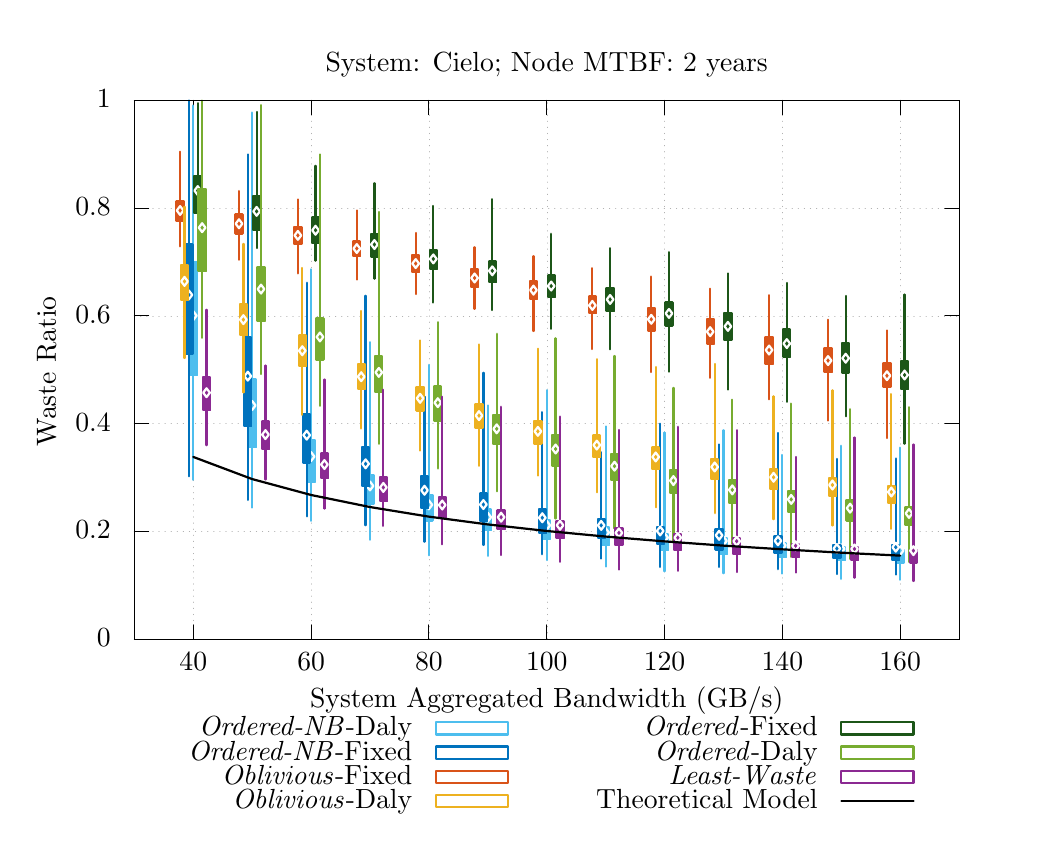
\begin{tikzpicture}[gnuplot]
%% generated with GNUPLOT 5.0p6 (Lua 5.3; terminal rev. 99, script rev. 100)
%% Thu Oct 19 13:54:21 2017
\path (0.000,0.000) rectangle (12.500,8.750);
\gpcolor{color=gp lt color axes}
\gpsetlinetype{gp lt axes}
\gpsetdashtype{gp dt axes}
\gpsetlinewidth{0.50}
\draw[gp path] (1.320,0.985)--(11.793,0.985);
\gpcolor{color=gp lt color border}
\gpsetlinetype{gp lt border}
\gpsetdashtype{gp dt solid}
\gpsetlinewidth{1.00}
\draw[gp path] (1.320,0.985)--(1.500,0.985);
\draw[gp path] (11.793,0.985)--(11.613,0.985);
\node[gp node right] at (1.136,0.985) {$0$};
\gpcolor{color=gp lt color axes}
\gpsetlinetype{gp lt axes}
\gpsetdashtype{gp dt axes}
\gpsetlinewidth{0.50}
\draw[gp path] (1.320,2.353)--(11.793,2.353);
\gpcolor{color=gp lt color border}
\gpsetlinetype{gp lt border}
\gpsetdashtype{gp dt solid}
\gpsetlinewidth{1.00}
\draw[gp path] (1.320,2.353)--(1.500,2.353);
\draw[gp path] (11.793,2.353)--(11.613,2.353);
\node[gp node right] at (1.136,2.353) {$0.2$};
\gpcolor{color=gp lt color axes}
\gpsetlinetype{gp lt axes}
\gpsetdashtype{gp dt axes}
\gpsetlinewidth{0.50}
\draw[gp path] (1.320,3.721)--(11.793,3.721);
\gpcolor{color=gp lt color border}
\gpsetlinetype{gp lt border}
\gpsetdashtype{gp dt solid}
\gpsetlinewidth{1.00}
\draw[gp path] (1.320,3.721)--(1.500,3.721);
\draw[gp path] (11.793,3.721)--(11.613,3.721);
\node[gp node right] at (1.136,3.721) {$0.4$};
\gpcolor{color=gp lt color axes}
\gpsetlinetype{gp lt axes}
\gpsetdashtype{gp dt axes}
\gpsetlinewidth{0.50}
\draw[gp path] (1.320,5.089)--(11.793,5.089);
\gpcolor{color=gp lt color border}
\gpsetlinetype{gp lt border}
\gpsetdashtype{gp dt solid}
\gpsetlinewidth{1.00}
\draw[gp path] (1.320,5.089)--(1.500,5.089);
\draw[gp path] (11.793,5.089)--(11.613,5.089);
\node[gp node right] at (1.136,5.089) {$0.6$};
\gpcolor{color=gp lt color axes}
\gpsetlinetype{gp lt axes}
\gpsetdashtype{gp dt axes}
\gpsetlinewidth{0.50}
\draw[gp path] (1.320,6.457)--(11.793,6.457);
\gpcolor{color=gp lt color border}
\gpsetlinetype{gp lt border}
\gpsetdashtype{gp dt solid}
\gpsetlinewidth{1.00}
\draw[gp path] (1.320,6.457)--(1.500,6.457);
\draw[gp path] (11.793,6.457)--(11.613,6.457);
\node[gp node right] at (1.136,6.457) {$0.8$};
\gpcolor{color=gp lt color axes}
\gpsetlinetype{gp lt axes}
\gpsetdashtype{gp dt axes}
\gpsetlinewidth{0.50}
\draw[gp path] (1.320,7.825)--(11.793,7.825);
\gpcolor{color=gp lt color border}
\gpsetlinetype{gp lt border}
\gpsetdashtype{gp dt solid}
\gpsetlinewidth{1.00}
\draw[gp path] (1.320,7.825)--(1.500,7.825);
\draw[gp path] (11.793,7.825)--(11.613,7.825);
\node[gp node right] at (1.136,7.825) {$1$};
\gpcolor{color=gp lt color axes}
\gpsetlinetype{gp lt axes}
\gpsetdashtype{gp dt axes}
\gpsetlinewidth{0.50}
\draw[gp path] (2.068,0.985)--(2.068,7.825);
\gpcolor{color=gp lt color border}
\gpsetlinetype{gp lt border}
\gpsetdashtype{gp dt solid}
\gpsetlinewidth{1.00}
\draw[gp path] (2.068,0.985)--(2.068,1.165);
\draw[gp path] (2.068,7.825)--(2.068,7.645);
\node[gp node center] at (2.068,0.677) {$40$};
\gpcolor{color=gp lt color axes}
\gpsetlinetype{gp lt axes}
\gpsetdashtype{gp dt axes}
\gpsetlinewidth{0.50}
\draw[gp path] (3.564,0.985)--(3.564,7.825);
\gpcolor{color=gp lt color border}
\gpsetlinetype{gp lt border}
\gpsetdashtype{gp dt solid}
\gpsetlinewidth{1.00}
\draw[gp path] (3.564,0.985)--(3.564,1.165);
\draw[gp path] (3.564,7.825)--(3.564,7.645);
\node[gp node center] at (3.564,0.677) {$60$};
\gpcolor{color=gp lt color axes}
\gpsetlinetype{gp lt axes}
\gpsetdashtype{gp dt axes}
\gpsetlinewidth{0.50}
\draw[gp path] (5.060,0.985)--(5.060,7.825);
\gpcolor{color=gp lt color border}
\gpsetlinetype{gp lt border}
\gpsetdashtype{gp dt solid}
\gpsetlinewidth{1.00}
\draw[gp path] (5.060,0.985)--(5.060,1.165);
\draw[gp path] (5.060,7.825)--(5.060,7.645);
\node[gp node center] at (5.060,0.677) {$80$};
\gpcolor{color=gp lt color axes}
\gpsetlinetype{gp lt axes}
\gpsetdashtype{gp dt axes}
\gpsetlinewidth{0.50}
\draw[gp path] (6.557,0.985)--(6.557,7.825);
\gpcolor{color=gp lt color border}
\gpsetlinetype{gp lt border}
\gpsetdashtype{gp dt solid}
\gpsetlinewidth{1.00}
\draw[gp path] (6.557,0.985)--(6.557,1.165);
\draw[gp path] (6.557,7.825)--(6.557,7.645);
\node[gp node center] at (6.557,0.677) {$100$};
\gpcolor{color=gp lt color axes}
\gpsetlinetype{gp lt axes}
\gpsetdashtype{gp dt axes}
\gpsetlinewidth{0.50}
\draw[gp path] (8.053,0.985)--(8.053,7.825);
\gpcolor{color=gp lt color border}
\gpsetlinetype{gp lt border}
\gpsetdashtype{gp dt solid}
\gpsetlinewidth{1.00}
\draw[gp path] (8.053,0.985)--(8.053,1.165);
\draw[gp path] (8.053,7.825)--(8.053,7.645);
\node[gp node center] at (8.053,0.677) {$120$};
\gpcolor{color=gp lt color axes}
\gpsetlinetype{gp lt axes}
\gpsetdashtype{gp dt axes}
\gpsetlinewidth{0.50}
\draw[gp path] (9.549,0.985)--(9.549,7.825);
\gpcolor{color=gp lt color border}
\gpsetlinetype{gp lt border}
\gpsetdashtype{gp dt solid}
\gpsetlinewidth{1.00}
\draw[gp path] (9.549,0.985)--(9.549,1.165);
\draw[gp path] (9.549,7.825)--(9.549,7.645);
\node[gp node center] at (9.549,0.677) {$140$};
\gpcolor{color=gp lt color axes}
\gpsetlinetype{gp lt axes}
\gpsetdashtype{gp dt axes}
\gpsetlinewidth{0.50}
\draw[gp path] (11.045,0.985)--(11.045,7.825);
\gpcolor{color=gp lt color border}
\gpsetlinetype{gp lt border}
\gpsetdashtype{gp dt solid}
\gpsetlinewidth{1.00}
\draw[gp path] (11.045,0.985)--(11.045,1.165);
\draw[gp path] (11.045,7.825)--(11.045,7.645);
\node[gp node center] at (11.045,0.677) {$160$};
\draw[gp path] (1.320,7.825)--(1.320,0.985)--(11.793,0.985)--(11.793,7.825)--cycle;
\node[gp node center,rotate=-270] at (0.246,4.405) {Waste Ratio};
\node[gp node center] at (6.556,0.215) {System Aggregated Bandwidth (GB/s)};
\node[gp node center] at (6.556,8.287) {System: Cielo; Node MTBF: 2 years};
\node[gp node right] at (4.966,-0.149) {\fifodaly};
\gpcolor{rgb color={0.302,0.745,0.933}}
\gpsetlinewidth{2.00}
\draw[gp path] (5.150,-0.226)--(6.066,-0.226)--(6.066,-0.072)--(5.150,-0.072)--cycle;
\gpfill{rgb color={0.302,0.745,0.933}} (2.023,4.342)--(2.113,4.342)--(2.113,5.777)--(2.023,5.777)--cycle;
\draw[gp path] (2.068,3.009)--(2.068,4.342);
\draw[gp path] (2.068,5.777)--(2.068,7.761);
\draw[gp path] (2.023,5.777)--(2.113,5.777)--(2.113,4.342)--(2.023,4.342)--cycle;
\gpfill{rgb color={0.302,0.745,0.933}} (2.771,3.427)--(2.861,3.427)--(2.861,4.281)--(2.771,4.281)--cycle;
\draw[gp path] (2.816,2.655)--(2.816,3.427);
\draw[gp path] (2.816,4.281)--(2.816,7.672);
\draw[gp path] (2.771,4.281)--(2.861,4.281)--(2.861,3.427)--(2.771,3.427)--cycle;
\gpfill{rgb color={0.302,0.745,0.933}} (3.519,2.985)--(3.609,2.985)--(3.609,3.514)--(3.519,3.514)--cycle;
\draw[gp path] (3.564,2.487)--(3.564,2.985);
\draw[gp path] (3.564,3.514)--(3.564,5.681);
\draw[gp path] (3.519,3.514)--(3.609,3.514)--(3.609,2.985)--(3.519,2.985)--cycle;
\gpfill{rgb color={0.302,0.745,0.933}} (4.267,2.696)--(4.357,2.696)--(4.357,3.073)--(4.267,3.073)--cycle;
\draw[gp path] (4.312,2.247)--(4.312,2.696);
\draw[gp path] (4.312,3.073)--(4.312,4.755);
\draw[gp path] (4.267,3.073)--(4.357,3.073)--(4.357,2.696)--(4.267,2.696)--cycle;
\gpfill{rgb color={0.302,0.745,0.933}} (5.015,2.491)--(5.105,2.491)--(5.105,2.819)--(5.015,2.819)--cycle;
\draw[gp path] (5.060,2.049)--(5.060,2.491);
\draw[gp path] (5.060,2.819)--(5.060,4.468);
\draw[gp path] (5.015,2.819)--(5.105,2.819)--(5.105,2.491)--(5.015,2.491)--cycle;
\gpfill{rgb color={0.302,0.745,0.933}} (5.763,2.372)--(5.853,2.372)--(5.853,2.631)--(5.763,2.631)--cycle;
\draw[gp path] (5.808,2.041)--(5.808,2.372);
\draw[gp path] (5.808,2.631)--(5.808,3.952);
\draw[gp path] (5.763,2.631)--(5.853,2.631)--(5.853,2.372)--(5.763,2.372)--cycle;
\gpfill{rgb color={0.302,0.745,0.933}} (6.512,2.260)--(6.602,2.260)--(6.602,2.501)--(6.512,2.501)--cycle;
\draw[gp path] (6.557,1.989)--(6.557,2.260);
\draw[gp path] (6.557,2.501)--(6.557,4.145);
\draw[gp path] (6.512,2.501)--(6.602,2.501)--(6.602,2.260)--(6.512,2.260)--cycle;
\gpfill{rgb color={0.302,0.745,0.933}} (7.260,2.175)--(7.350,2.175)--(7.350,2.406)--(7.260,2.406)--cycle;
\draw[gp path] (7.305,1.906)--(7.305,2.175);
\draw[gp path] (7.305,2.406)--(7.305,3.686);
\draw[gp path] (7.260,2.406)--(7.350,2.406)--(7.350,2.175)--(7.260,2.175)--cycle;
\gpfill{rgb color={0.302,0.745,0.933}} (8.008,2.117)--(8.098,2.117)--(8.098,2.319)--(8.008,2.319)--cycle;
\draw[gp path] (8.053,1.846)--(8.053,2.117);
\draw[gp path] (8.053,2.319)--(8.053,3.608);
\draw[gp path] (8.008,2.319)--(8.098,2.319)--(8.098,2.117)--(8.008,2.117)--cycle;
\gpfill{rgb color={0.302,0.745,0.933}} (8.756,2.068)--(8.846,2.068)--(8.846,2.265)--(8.756,2.265)--cycle;
\draw[gp path] (8.801,1.821)--(8.801,2.068);
\draw[gp path] (8.801,2.265)--(8.801,3.638);
\draw[gp path] (8.756,2.265)--(8.846,2.265)--(8.846,2.068)--(8.756,2.068)--cycle;
\gpfill{rgb color={0.302,0.745,0.933}} (9.504,2.026)--(9.594,2.026)--(9.594,2.199)--(9.504,2.199)--cycle;
\draw[gp path] (9.549,1.817)--(9.549,2.026);
\draw[gp path] (9.549,2.199)--(9.549,3.324);
\draw[gp path] (9.504,2.199)--(9.594,2.199)--(9.594,2.026)--(9.504,2.026)--cycle;
\gpfill{rgb color={0.302,0.745,0.933}} (10.252,1.985)--(10.342,1.985)--(10.342,2.157)--(10.252,2.157)--cycle;
\draw[gp path] (10.297,1.749)--(10.297,1.985);
\draw[gp path] (10.297,2.157)--(10.297,3.440);
\draw[gp path] (10.252,2.157)--(10.342,2.157)--(10.342,1.985)--(10.252,1.985)--cycle;
\gpfill{rgb color={0.302,0.745,0.933}} (11.000,1.959)--(11.090,1.959)--(11.090,2.120)--(11.000,2.120)--cycle;
\draw[gp path] (11.045,1.739)--(11.045,1.959);
\draw[gp path] (11.045,2.120)--(11.045,3.417);
\draw[gp path] (11.000,2.120)--(11.090,2.120)--(11.090,1.959)--(11.000,1.959)--cycle;
\gpcolor{rgb color={1.000,1.000,1.000}}
\gpsetpointsize{4.00}
\gppoint{gp mark 12}{(2.068,5.093)}
\gppoint{gp mark 12}{(2.816,3.952)}
\gppoint{gp mark 12}{(3.564,3.303)}
\gppoint{gp mark 12}{(4.312,2.930)}
\gppoint{gp mark 12}{(5.060,2.690)}
\gppoint{gp mark 12}{(5.808,2.533)}
\gppoint{gp mark 12}{(6.557,2.430)}
\gppoint{gp mark 12}{(7.305,2.338)}
\gppoint{gp mark 12}{(8.053,2.274)}
\gppoint{gp mark 12}{(8.801,2.232)}
\gppoint{gp mark 12}{(9.549,2.174)}
\gppoint{gp mark 12}{(10.297,2.131)}
\gppoint{gp mark 12}{(11.045,2.110)}
\gpcolor{color=gp lt color border}
\node[gp node right] at (4.966,-0.457) {\fifofixed};
\gpcolor{rgb color={0.000,0.447,0.741}}
\draw[gp path] (5.150,-0.534)--(6.066,-0.534)--(6.066,-0.380)--(5.150,-0.380)--cycle;
\gpfill{rgb color={0.000,0.447,0.741}} (1.967,4.608)--(2.057,4.608)--(2.057,5.997)--(1.967,5.997)--cycle;
\draw[gp path] (2.012,3.053)--(2.012,4.608);
\draw[gp path] (2.012,5.997)--(2.012,7.825);
\draw[gp path] (1.967,5.997)--(2.057,5.997)--(2.057,4.608)--(1.967,4.608)--cycle;
\gpfill{rgb color={0.000,0.447,0.741}} (2.715,3.689)--(2.805,3.689)--(2.805,4.817)--(2.715,4.817)--cycle;
\draw[gp path] (2.760,2.752)--(2.760,3.689);
\draw[gp path] (2.760,4.817)--(2.760,7.139);
\draw[gp path] (2.715,4.817)--(2.805,4.817)--(2.805,3.689)--(2.715,3.689)--cycle;
\gpfill{rgb color={0.000,0.447,0.741}} (3.463,3.227)--(3.553,3.227)--(3.553,3.846)--(3.463,3.846)--cycle;
\draw[gp path] (3.508,2.543)--(3.508,3.227);
\draw[gp path] (3.508,3.846)--(3.508,5.510);
\draw[gp path] (3.463,3.846)--(3.553,3.846)--(3.553,3.227)--(3.463,3.227)--cycle;
\gpfill{rgb color={0.000,0.447,0.741}} (4.211,2.932)--(4.301,2.932)--(4.301,3.422)--(4.211,3.422)--cycle;
\draw[gp path] (4.256,2.430)--(4.256,2.932);
\draw[gp path] (4.256,3.422)--(4.256,5.345);
\draw[gp path] (4.211,3.422)--(4.301,3.422)--(4.301,2.932)--(4.211,2.932)--cycle;
\gpfill{rgb color={0.000,0.447,0.741}} (4.959,2.648)--(5.049,2.648)--(5.049,3.053)--(4.959,3.053)--cycle;
\draw[gp path] (5.004,2.221)--(5.004,2.648);
\draw[gp path] (5.004,3.053)--(5.004,4.064);
\draw[gp path] (4.959,3.053)--(5.049,3.053)--(5.049,2.648)--(4.959,2.648)--cycle;
\gpfill{rgb color={0.000,0.447,0.741}} (5.707,2.486)--(5.797,2.486)--(5.797,2.834)--(5.707,2.834)--cycle;
\draw[gp path] (5.752,2.180)--(5.752,2.486);
\draw[gp path] (5.752,2.834)--(5.752,4.367);
\draw[gp path] (5.707,2.834)--(5.797,2.834)--(5.797,2.486)--(5.707,2.486)--cycle;
\gpfill{rgb color={0.000,0.447,0.741}} (6.455,2.334)--(6.545,2.334)--(6.545,2.636)--(6.455,2.636)--cycle;
\draw[gp path] (6.500,2.063)--(6.500,2.334);
\draw[gp path] (6.500,2.636)--(6.500,3.868);
\draw[gp path] (6.455,2.636)--(6.545,2.636)--(6.545,2.334)--(6.455,2.334)--cycle;
\gpfill{rgb color={0.000,0.447,0.741}} (7.203,2.265)--(7.293,2.265)--(7.293,2.514)--(7.203,2.514)--cycle;
\draw[gp path] (7.248,2.007)--(7.248,2.265);
\draw[gp path] (7.248,2.514)--(7.248,3.360);
\draw[gp path] (7.203,2.514)--(7.293,2.514)--(7.293,2.265)--(7.203,2.265)--cycle;
\gpfill{rgb color={0.000,0.447,0.741}} (7.952,2.197)--(8.042,2.197)--(8.042,2.412)--(7.952,2.412)--cycle;
\draw[gp path] (7.997,1.901)--(7.997,2.197);
\draw[gp path] (7.997,2.412)--(7.997,3.720);
\draw[gp path] (7.952,2.412)--(8.042,2.412)--(8.042,2.197)--(7.952,2.197)--cycle;
\gpfill{rgb color={0.000,0.447,0.741}} (8.700,2.123)--(8.790,2.123)--(8.790,2.382)--(8.700,2.382)--cycle;
\draw[gp path] (8.745,1.901)--(8.745,2.123);
\draw[gp path] (8.745,2.382)--(8.745,3.457);
\draw[gp path] (8.700,2.382)--(8.790,2.382)--(8.790,2.123)--(8.700,2.123)--cycle;
\gpfill{rgb color={0.000,0.447,0.741}} (9.448,2.080)--(9.538,2.080)--(9.538,2.296)--(9.448,2.296)--cycle;
\draw[gp path] (9.493,1.873)--(9.493,2.080);
\draw[gp path] (9.493,2.296)--(9.493,3.603);
\draw[gp path] (9.448,2.296)--(9.538,2.296)--(9.538,2.080)--(9.448,2.080)--cycle;
\gpfill{rgb color={0.000,0.447,0.741}} (10.196,2.017)--(10.286,2.017)--(10.286,2.176)--(10.196,2.176)--cycle;
\draw[gp path] (10.241,1.811)--(10.241,2.017);
\draw[gp path] (10.241,2.176)--(10.241,3.274);
\draw[gp path] (10.196,2.176)--(10.286,2.176)--(10.286,2.017)--(10.196,2.017)--cycle;
\gpfill{rgb color={0.000,0.447,0.741}} (10.944,1.993)--(11.034,1.993)--(11.034,2.182)--(10.944,2.182)--cycle;
\draw[gp path] (10.989,1.805)--(10.989,1.993);
\draw[gp path] (10.989,2.182)--(10.989,3.278);
\draw[gp path] (10.944,2.182)--(11.034,2.182)--(11.034,1.993)--(10.944,1.993)--cycle;
\gpcolor{rgb color={1.000,1.000,1.000}}
\gppoint{gp mark 12}{(2.012,5.356)}
\gppoint{gp mark 12}{(2.760,4.324)}
\gppoint{gp mark 12}{(3.508,3.575)}
\gppoint{gp mark 12}{(4.256,3.211)}
\gppoint{gp mark 12}{(5.004,2.875)}
\gppoint{gp mark 12}{(5.752,2.694)}
\gppoint{gp mark 12}{(6.500,2.526)}
\gppoint{gp mark 12}{(7.248,2.429)}
\gppoint{gp mark 12}{(7.997,2.358)}
\gppoint{gp mark 12}{(8.745,2.303)}
\gppoint{gp mark 12}{(9.493,2.233)}
\gppoint{gp mark 12}{(10.241,2.135)}
\gppoint{gp mark 12}{(10.989,2.152)}
\gpcolor{color=gp lt color border}
\node[gp node right] at (4.966,-0.765) {\propfixed};
\gpcolor{rgb color={0.851,0.325,0.098}}
\draw[gp path] (5.150,-0.842)--(6.066,-0.842)--(6.066,-0.688)--(5.150,-0.688)--cycle;
\gpfill{rgb color={0.851,0.325,0.098}} (1.855,6.295)--(1.945,6.295)--(1.945,6.541)--(1.855,6.541)--cycle;
\draw[gp path] (1.900,5.972)--(1.900,6.295);
\draw[gp path] (1.900,6.541)--(1.900,7.174);
\draw[gp path] (1.855,6.541)--(1.945,6.541)--(1.945,6.295)--(1.855,6.295)--cycle;
\gpfill{rgb color={0.851,0.325,0.098}} (2.603,6.137)--(2.693,6.137)--(2.693,6.377)--(2.603,6.377)--cycle;
\draw[gp path] (2.648,5.803)--(2.648,6.137);
\draw[gp path] (2.648,6.377)--(2.648,6.675);
\draw[gp path] (2.603,6.377)--(2.693,6.377)--(2.693,6.137)--(2.603,6.137)--cycle;
\gpfill{rgb color={0.851,0.325,0.098}} (3.351,6.001)--(3.441,6.001)--(3.441,6.215)--(3.351,6.215)--cycle;
\draw[gp path] (3.396,5.629)--(3.396,6.001);
\draw[gp path] (3.396,6.215)--(3.396,6.569);
\draw[gp path] (3.351,6.215)--(3.441,6.215)--(3.441,6.001)--(3.351,6.001)--cycle;
\gpfill{rgb color={0.851,0.325,0.098}} (4.099,5.847)--(4.189,5.847)--(4.189,6.035)--(4.099,6.035)--cycle;
\draw[gp path] (4.144,5.550)--(4.144,5.847);
\draw[gp path] (4.144,6.035)--(4.144,6.428);
\draw[gp path] (4.099,6.035)--(4.189,6.035)--(4.189,5.847)--(4.099,5.847)--cycle;
\gpfill{rgb color={0.851,0.325,0.098}} (4.847,5.648)--(4.937,5.648)--(4.937,5.863)--(4.847,5.863)--cycle;
\draw[gp path] (4.892,5.367)--(4.892,5.648);
\draw[gp path] (4.892,5.863)--(4.892,6.143);
\draw[gp path] (4.847,5.863)--(4.937,5.863)--(4.937,5.648)--(4.847,5.648)--cycle;
\gpfill{rgb color={0.851,0.325,0.098}} (5.595,5.461)--(5.685,5.461)--(5.685,5.682)--(5.595,5.682)--cycle;
\draw[gp path] (5.640,5.179)--(5.640,5.461);
\draw[gp path] (5.640,5.682)--(5.640,5.962);
\draw[gp path] (5.595,5.682)--(5.685,5.682)--(5.685,5.461)--(5.595,5.461)--cycle;
\gpfill{rgb color={0.851,0.325,0.098}} (6.343,5.309)--(6.433,5.309)--(6.433,5.535)--(6.343,5.535)--cycle;
\draw[gp path] (6.388,4.897)--(6.388,5.309);
\draw[gp path] (6.388,5.535)--(6.388,5.848);
\draw[gp path] (6.343,5.535)--(6.433,5.535)--(6.433,5.309)--(6.343,5.309)--cycle;
\gpfill{rgb color={0.851,0.325,0.098}} (7.091,5.123)--(7.181,5.123)--(7.181,5.335)--(7.091,5.335)--cycle;
\draw[gp path] (7.136,4.669)--(7.136,5.123);
\draw[gp path] (7.136,5.335)--(7.136,5.696);
\draw[gp path] (7.091,5.335)--(7.181,5.335)--(7.181,5.123)--(7.091,5.123)--cycle;
\gpfill{rgb color={0.851,0.325,0.098}} (7.839,4.905)--(7.929,4.905)--(7.929,5.191)--(7.839,5.191)--cycle;
\draw[gp path] (7.884,4.377)--(7.884,4.905);
\draw[gp path] (7.884,5.191)--(7.884,5.589);
\draw[gp path] (7.839,5.191)--(7.929,5.191)--(7.929,4.905)--(7.839,4.905)--cycle;
\gpfill{rgb color={0.851,0.325,0.098}} (8.587,4.738)--(8.677,4.738)--(8.677,5.054)--(8.587,5.054)--cycle;
\draw[gp path] (8.632,4.303)--(8.632,4.738);
\draw[gp path] (8.632,5.054)--(8.632,5.435);
\draw[gp path] (8.587,5.054)--(8.677,5.054)--(8.677,4.738)--(8.587,4.738)--cycle;
\gpfill{rgb color={0.851,0.325,0.098}} (9.335,4.482)--(9.425,4.482)--(9.425,4.824)--(9.335,4.824)--cycle;
\draw[gp path] (9.380,4.030)--(9.380,4.482);
\draw[gp path] (9.380,4.824)--(9.380,5.353);
\draw[gp path] (9.335,4.824)--(9.425,4.824)--(9.425,4.482)--(9.335,4.482)--cycle;
\gpfill{rgb color={0.851,0.325,0.098}} (10.084,4.379)--(10.174,4.379)--(10.174,4.681)--(10.084,4.681)--cycle;
\draw[gp path] (10.129,3.761)--(10.129,4.379);
\draw[gp path] (10.129,4.681)--(10.129,5.041);
\draw[gp path] (10.084,4.681)--(10.174,4.681)--(10.174,4.379)--(10.084,4.379)--cycle;
\gpfill{rgb color={0.851,0.325,0.098}} (10.832,4.183)--(10.922,4.183)--(10.922,4.487)--(10.832,4.487)--cycle;
\draw[gp path] (10.877,3.539)--(10.877,4.183);
\draw[gp path] (10.877,4.487)--(10.877,4.904);
\draw[gp path] (10.832,4.487)--(10.922,4.487)--(10.922,4.183)--(10.832,4.183)--cycle;
\gpcolor{rgb color={1.000,1.000,1.000}}
\gppoint{gp mark 12}{(1.900,6.428)}
\gppoint{gp mark 12}{(2.648,6.260)}
\gppoint{gp mark 12}{(3.396,6.112)}
\gppoint{gp mark 12}{(4.144,5.945)}
\gppoint{gp mark 12}{(4.892,5.754)}
\gppoint{gp mark 12}{(5.640,5.571)}
\gppoint{gp mark 12}{(6.388,5.417)}
\gppoint{gp mark 12}{(7.136,5.222)}
\gppoint{gp mark 12}{(7.884,5.046)}
\gppoint{gp mark 12}{(8.632,4.889)}
\gppoint{gp mark 12}{(9.380,4.656)}
\gppoint{gp mark 12}{(10.129,4.522)}
\gppoint{gp mark 12}{(10.877,4.330)}
\gpcolor{color=gp lt color border}
\node[gp node right] at (4.966,-1.073) {\propdaly};
\gpcolor{rgb color={0.929,0.694,0.125}}
\draw[gp path] (5.150,-1.150)--(6.066,-1.150)--(6.066,-0.996)--(5.150,-0.996)--cycle;
\gpfill{rgb color={0.929,0.694,0.125}} (1.911,5.296)--(2.001,5.296)--(2.001,5.740)--(1.911,5.740)--cycle;
\draw[gp path] (1.956,4.554)--(1.956,5.296);
\draw[gp path] (1.956,5.740)--(1.956,6.476);
\draw[gp path] (1.911,5.740)--(2.001,5.740)--(2.001,5.296)--(1.911,5.296)--cycle;
\gpfill{rgb color={0.929,0.694,0.125}} (2.659,4.847)--(2.749,4.847)--(2.749,5.241)--(2.659,5.241)--cycle;
\draw[gp path] (2.704,4.117)--(2.704,4.847);
\draw[gp path] (2.704,5.241)--(2.704,6.004);
\draw[gp path] (2.659,5.241)--(2.749,5.241)--(2.749,4.847)--(2.659,4.847)--cycle;
\gpfill{rgb color={0.929,0.694,0.125}} (3.407,4.456)--(3.497,4.456)--(3.497,4.840)--(3.407,4.840)--cycle;
\draw[gp path] (3.452,3.834)--(3.452,4.456);
\draw[gp path] (3.452,4.840)--(3.452,5.698);
\draw[gp path] (3.407,4.840)--(3.497,4.840)--(3.497,4.456)--(3.407,4.456)--cycle;
\gpfill{rgb color={0.929,0.694,0.125}} (4.155,4.159)--(4.245,4.159)--(4.245,4.479)--(4.155,4.479)--cycle;
\draw[gp path] (4.200,3.660)--(4.200,4.159);
\draw[gp path] (4.200,4.479)--(4.200,5.153);
\draw[gp path] (4.155,4.479)--(4.245,4.479)--(4.245,4.159)--(4.155,4.159)--cycle;
\gpfill{rgb color={0.929,0.694,0.125}} (4.903,3.888)--(4.993,3.888)--(4.993,4.191)--(4.903,4.191)--cycle;
\draw[gp path] (4.948,3.379)--(4.948,3.888);
\draw[gp path] (4.948,4.191)--(4.948,4.778);
\draw[gp path] (4.903,4.191)--(4.993,4.191)--(4.993,3.888)--(4.903,3.888)--cycle;
\gpfill{rgb color={0.929,0.694,0.125}} (5.651,3.667)--(5.741,3.667)--(5.741,3.973)--(5.651,3.973)--cycle;
\draw[gp path] (5.696,3.185)--(5.696,3.667);
\draw[gp path] (5.696,3.973)--(5.696,4.726);
\draw[gp path] (5.651,3.973)--(5.741,3.973)--(5.741,3.667)--(5.651,3.667)--cycle;
\gpfill{rgb color={0.929,0.694,0.125}} (6.399,3.469)--(6.489,3.469)--(6.489,3.759)--(6.399,3.759)--cycle;
\draw[gp path] (6.444,3.061)--(6.444,3.469);
\draw[gp path] (6.444,3.759)--(6.444,4.674);
\draw[gp path] (6.399,3.759)--(6.489,3.759)--(6.489,3.469)--(6.399,3.469)--cycle;
\gpfill{rgb color={0.929,0.694,0.125}} (7.147,3.299)--(7.237,3.299)--(7.237,3.571)--(7.147,3.571)--cycle;
\draw[gp path] (7.192,2.850)--(7.192,3.299);
\draw[gp path] (7.192,3.571)--(7.192,4.540);
\draw[gp path] (7.147,3.571)--(7.237,3.571)--(7.237,3.299)--(7.147,3.299)--cycle;
\gpfill{rgb color={0.929,0.694,0.125}} (7.895,3.146)--(7.985,3.146)--(7.985,3.418)--(7.895,3.418)--cycle;
\draw[gp path] (7.940,2.659)--(7.940,3.146);
\draw[gp path] (7.940,3.418)--(7.940,4.440);
\draw[gp path] (7.895,3.418)--(7.985,3.418)--(7.985,3.146)--(7.895,3.146)--cycle;
\gpfill{rgb color={0.929,0.694,0.125}} (8.644,3.015)--(8.734,3.015)--(8.734,3.274)--(8.644,3.274)--cycle;
\draw[gp path] (8.689,2.584)--(8.689,3.015);
\draw[gp path] (8.689,3.274)--(8.689,4.480);
\draw[gp path] (8.644,3.274)--(8.734,3.274)--(8.734,3.015)--(8.644,3.015)--cycle;
\gpfill{rgb color={0.929,0.694,0.125}} (9.392,2.894)--(9.482,2.894)--(9.482,3.141)--(9.392,3.141)--cycle;
\draw[gp path] (9.437,2.507)--(9.437,2.894);
\draw[gp path] (9.437,3.141)--(9.437,4.068);
\draw[gp path] (9.392,3.141)--(9.482,3.141)--(9.482,2.894)--(9.392,2.894)--cycle;
\gpfill{rgb color={0.929,0.694,0.125}} (10.140,2.799)--(10.230,2.799)--(10.230,3.032)--(10.140,3.032)--cycle;
\draw[gp path] (10.185,2.427)--(10.185,2.799);
\draw[gp path] (10.185,3.032)--(10.185,4.144);
\draw[gp path] (10.140,3.032)--(10.230,3.032)--(10.230,2.799)--(10.140,2.799)--cycle;
\gpfill{rgb color={0.929,0.694,0.125}} (10.888,2.714)--(10.978,2.714)--(10.978,2.929)--(10.888,2.929)--cycle;
\draw[gp path] (10.933,2.386)--(10.933,2.714);
\draw[gp path] (10.933,2.929)--(10.933,4.097);
\draw[gp path] (10.888,2.929)--(10.978,2.929)--(10.978,2.714)--(10.888,2.714)--cycle;
\gpcolor{rgb color={1.000,1.000,1.000}}
\gppoint{gp mark 12}{(1.956,5.528)}
\gppoint{gp mark 12}{(2.704,5.042)}
\gppoint{gp mark 12}{(3.452,4.647)}
\gppoint{gp mark 12}{(4.200,4.317)}
\gppoint{gp mark 12}{(4.948,4.043)}
\gppoint{gp mark 12}{(5.696,3.823)}
\gppoint{gp mark 12}{(6.444,3.623)}
\gppoint{gp mark 12}{(7.192,3.449)}
\gppoint{gp mark 12}{(7.940,3.298)}
\gppoint{gp mark 12}{(8.689,3.171)}
\gppoint{gp mark 12}{(9.437,3.040)}
\gppoint{gp mark 12}{(10.185,2.942)}
\gppoint{gp mark 12}{(10.933,2.853)}
\gpcolor{color=gp lt color border}
\node[gp node right] at (10.114,-0.149) {\bfifofixed};
\gpcolor{rgb color={0.110,0.337,0.094}}
\draw[gp path] (10.298,-0.226)--(11.214,-0.226)--(11.214,-0.072)--(10.298,-0.072)--cycle;
\gpfill{rgb color={0.110,0.337,0.094}} (2.079,6.397)--(2.169,6.397)--(2.169,6.864)--(2.079,6.864)--cycle;
\draw[gp path] (2.124,6.053)--(2.124,6.397);
\draw[gp path] (2.124,6.864)--(2.124,7.790);
\draw[gp path] (2.079,6.864)--(2.169,6.864)--(2.169,6.397)--(2.079,6.397)--cycle;
\gpfill{rgb color={0.110,0.337,0.094}} (2.827,6.180)--(2.917,6.180)--(2.917,6.608)--(2.827,6.608)--cycle;
\draw[gp path] (2.872,5.950)--(2.872,6.180);
\draw[gp path] (2.872,6.608)--(2.872,7.680);
\draw[gp path] (2.827,6.608)--(2.917,6.608)--(2.917,6.180)--(2.827,6.180)--cycle;
\gpfill{rgb color={0.110,0.337,0.094}} (3.575,6.011)--(3.665,6.011)--(3.665,6.339)--(3.575,6.339)--cycle;
\draw[gp path] (3.620,5.791)--(3.620,6.011);
\draw[gp path] (3.620,6.339)--(3.620,6.995);
\draw[gp path] (3.575,6.339)--(3.665,6.339)--(3.665,6.011)--(3.575,6.011)--cycle;
\gpfill{rgb color={0.110,0.337,0.094}} (4.323,5.844)--(4.413,5.844)--(4.413,6.125)--(4.323,6.125)--cycle;
\draw[gp path] (4.368,5.562)--(4.368,5.844);
\draw[gp path] (4.368,6.125)--(4.368,6.775);
\draw[gp path] (4.323,6.125)--(4.413,6.125)--(4.413,5.844)--(4.323,5.844)--cycle;
\gpfill{rgb color={0.110,0.337,0.094}} (5.071,5.690)--(5.161,5.690)--(5.161,5.930)--(5.071,5.930)--cycle;
\draw[gp path] (5.116,5.260)--(5.116,5.690);
\draw[gp path] (5.116,5.930)--(5.116,6.485);
\draw[gp path] (5.071,5.930)--(5.161,5.930)--(5.161,5.690)--(5.071,5.690)--cycle;
\gpfill{rgb color={0.110,0.337,0.094}} (5.820,5.522)--(5.910,5.522)--(5.910,5.781)--(5.820,5.781)--cycle;
\draw[gp path] (5.865,5.164)--(5.865,5.522);
\draw[gp path] (5.865,5.781)--(5.865,6.571);
\draw[gp path] (5.820,5.781)--(5.910,5.781)--(5.910,5.522)--(5.820,5.522)--cycle;
\gpfill{rgb color={0.110,0.337,0.094}} (6.568,5.331)--(6.658,5.331)--(6.658,5.602)--(6.568,5.602)--cycle;
\draw[gp path] (6.613,4.926)--(6.613,5.331);
\draw[gp path] (6.613,5.602)--(6.613,6.132);
\draw[gp path] (6.568,5.602)--(6.658,5.602)--(6.658,5.331)--(6.568,5.331)--cycle;
\gpfill{rgb color={0.110,0.337,0.094}} (7.316,5.147)--(7.406,5.147)--(7.406,5.441)--(7.316,5.441)--cycle;
\draw[gp path] (7.361,4.666)--(7.361,5.147);
\draw[gp path] (7.361,5.441)--(7.361,5.950);
\draw[gp path] (7.316,5.441)--(7.406,5.441)--(7.406,5.147)--(7.316,5.147)--cycle;
\gpfill{rgb color={0.110,0.337,0.094}} (8.064,4.967)--(8.154,4.967)--(8.154,5.259)--(8.064,5.259)--cycle;
\draw[gp path] (8.109,4.381)--(8.109,4.967);
\draw[gp path] (8.109,5.259)--(8.109,5.900);
\draw[gp path] (8.064,5.259)--(8.154,5.259)--(8.154,4.967)--(8.064,4.967)--cycle;
\gpfill{rgb color={0.110,0.337,0.094}} (8.812,4.785)--(8.902,4.785)--(8.902,5.130)--(8.812,5.130)--cycle;
\draw[gp path] (8.857,4.153)--(8.857,4.785);
\draw[gp path] (8.857,5.130)--(8.857,5.629);
\draw[gp path] (8.812,5.130)--(8.902,5.130)--(8.902,4.785)--(8.812,4.785)--cycle;
\gpfill{rgb color={0.110,0.337,0.094}} (9.560,4.573)--(9.650,4.573)--(9.650,4.917)--(9.560,4.917)--cycle;
\draw[gp path] (9.605,3.998)--(9.605,4.573);
\draw[gp path] (9.605,4.917)--(9.605,5.508);
\draw[gp path] (9.560,4.917)--(9.650,4.917)--(9.650,4.573)--(9.560,4.573)--cycle;
\gpfill{rgb color={0.110,0.337,0.094}} (10.308,4.370)--(10.398,4.370)--(10.398,4.744)--(10.308,4.744)--cycle;
\draw[gp path] (10.353,3.814)--(10.353,4.370);
\draw[gp path] (10.353,4.744)--(10.353,5.343);
\draw[gp path] (10.308,4.744)--(10.398,4.744)--(10.398,4.370)--(10.308,4.370)--cycle;
\gpfill{rgb color={0.110,0.337,0.094}} (11.056,4.158)--(11.146,4.158)--(11.146,4.520)--(11.056,4.520)--cycle;
\draw[gp path] (11.101,3.466)--(11.101,4.158);
\draw[gp path] (11.101,4.520)--(11.101,5.361);
\draw[gp path] (11.056,4.520)--(11.146,4.520)--(11.146,4.158)--(11.056,4.158)--cycle;
\gpcolor{rgb color={1.000,1.000,1.000}}
\gppoint{gp mark 12}{(2.124,6.681)}
\gppoint{gp mark 12}{(2.872,6.417)}
\gppoint{gp mark 12}{(3.620,6.177)}
\gppoint{gp mark 12}{(4.368,5.996)}
\gppoint{gp mark 12}{(5.116,5.813)}
\gppoint{gp mark 12}{(5.865,5.662)}
\gppoint{gp mark 12}{(6.613,5.469)}
\gppoint{gp mark 12}{(7.361,5.298)}
\gppoint{gp mark 12}{(8.109,5.121)}
\gppoint{gp mark 12}{(8.857,4.956)}
\gppoint{gp mark 12}{(9.605,4.738)}
\gppoint{gp mark 12}{(10.353,4.552)}
\gppoint{gp mark 12}{(11.101,4.339)}
\gpcolor{color=gp lt color border}
\node[gp node right] at (10.114,-0.457) {\bfifodaly};
\gpcolor{rgb color={0.467,0.675,0.188}}
\draw[gp path] (10.298,-0.534)--(11.214,-0.534)--(11.214,-0.380)--(10.298,-0.380)--cycle;
\gpfill{rgb color={0.467,0.675,0.188}} (2.135,5.660)--(2.225,5.660)--(2.225,6.697)--(2.135,6.697)--cycle;
\draw[gp path] (2.180,4.810)--(2.180,5.660);
\draw[gp path] (2.180,6.697)--(2.180,7.824);
\draw[gp path] (2.135,6.697)--(2.225,6.697)--(2.225,5.660)--(2.135,5.660)--cycle;
\gpfill{rgb color={0.467,0.675,0.188}} (2.883,5.027)--(2.973,5.027)--(2.973,5.706)--(2.883,5.706)--cycle;
\draw[gp path] (2.928,4.350)--(2.928,5.027);
\draw[gp path] (2.928,5.706)--(2.928,7.767);
\draw[gp path] (2.883,5.706)--(2.973,5.706)--(2.973,5.027)--(2.883,5.027)--cycle;
\gpfill{rgb color={0.467,0.675,0.188}} (3.631,4.536)--(3.721,4.536)--(3.721,5.057)--(3.631,5.057)--cycle;
\draw[gp path] (3.676,3.947)--(3.676,4.536);
\draw[gp path] (3.676,5.057)--(3.676,7.139);
\draw[gp path] (3.631,5.057)--(3.721,5.057)--(3.721,4.536)--(3.631,4.536)--cycle;
\gpfill{rgb color={0.467,0.675,0.188}} (4.379,4.121)--(4.469,4.121)--(4.469,4.584)--(4.379,4.584)--cycle;
\draw[gp path] (4.424,3.465)--(4.424,4.121);
\draw[gp path] (4.424,4.584)--(4.424,6.409);
\draw[gp path] (4.379,4.584)--(4.469,4.584)--(4.469,4.121)--(4.379,4.121)--cycle;
\gpfill{rgb color={0.467,0.675,0.188}} (5.128,3.761)--(5.218,3.761)--(5.218,4.192)--(5.128,4.192)--cycle;
\draw[gp path] (5.173,3.152)--(5.173,3.761);
\draw[gp path] (5.173,4.192)--(5.173,5.010);
\draw[gp path] (5.128,4.192)--(5.218,4.192)--(5.218,3.761)--(5.128,3.761)--cycle;
\gpfill{rgb color={0.467,0.675,0.188}} (5.876,3.466)--(5.966,3.466)--(5.966,3.830)--(5.876,3.830)--cycle;
\draw[gp path] (5.921,2.861)--(5.921,3.466);
\draw[gp path] (5.921,3.830)--(5.921,4.862);
\draw[gp path] (5.876,3.830)--(5.966,3.830)--(5.966,3.466)--(5.876,3.466)--cycle;
\gpfill{rgb color={0.467,0.675,0.188}} (6.624,3.189)--(6.714,3.189)--(6.714,3.574)--(6.624,3.574)--cycle;
\draw[gp path] (6.669,2.516)--(6.669,3.189);
\draw[gp path] (6.669,3.574)--(6.669,4.805);
\draw[gp path] (6.624,3.574)--(6.714,3.574)--(6.714,3.189)--(6.624,3.189)--cycle;
\gpfill{rgb color={0.467,0.675,0.188}} (7.372,3.002)--(7.462,3.002)--(7.462,3.332)--(7.372,3.332)--cycle;
\draw[gp path] (7.417,2.391)--(7.417,3.002);
\draw[gp path] (7.417,3.332)--(7.417,4.581);
\draw[gp path] (7.372,3.332)--(7.462,3.332)--(7.462,3.002)--(7.372,3.002)--cycle;
\gpfill{rgb color={0.467,0.675,0.188}} (8.120,2.838)--(8.210,2.838)--(8.210,3.129)--(8.120,3.129)--cycle;
\draw[gp path] (8.165,2.221)--(8.165,2.838);
\draw[gp path] (8.165,3.129)--(8.165,4.175);
\draw[gp path] (8.120,3.129)--(8.210,3.129)--(8.210,2.838)--(8.120,2.838)--cycle;
\gpfill{rgb color={0.467,0.675,0.188}} (8.868,2.709)--(8.958,2.709)--(8.958,3.004)--(8.868,3.004)--cycle;
\draw[gp path] (8.913,2.196)--(8.913,2.709);
\draw[gp path] (8.913,3.004)--(8.913,4.026);
\draw[gp path] (8.868,3.004)--(8.958,3.004)--(8.958,2.709)--(8.868,2.709)--cycle;
\gpfill{rgb color={0.467,0.675,0.188}} (9.616,2.596)--(9.706,2.596)--(9.706,2.865)--(9.616,2.865)--cycle;
\draw[gp path] (9.661,2.031)--(9.661,2.596);
\draw[gp path] (9.661,2.865)--(9.661,3.976);
\draw[gp path] (9.616,2.865)--(9.706,2.865)--(9.706,2.596)--(9.616,2.596)--cycle;
\gpfill{rgb color={0.467,0.675,0.188}} (10.364,2.491)--(10.454,2.491)--(10.454,2.751)--(10.364,2.751)--cycle;
\draw[gp path] (10.409,2.004)--(10.409,2.491);
\draw[gp path] (10.409,2.751)--(10.409,3.906);
\draw[gp path] (10.364,2.751)--(10.454,2.751)--(10.454,2.491)--(10.364,2.491)--cycle;
\gpfill{rgb color={0.467,0.675,0.188}} (11.112,2.431)--(11.202,2.431)--(11.202,2.667)--(11.112,2.667)--cycle;
\draw[gp path] (11.157,1.965)--(11.157,2.431);
\draw[gp path] (11.157,2.667)--(11.157,3.930);
\draw[gp path] (11.112,2.667)--(11.202,2.667)--(11.202,2.431)--(11.112,2.431)--cycle;
\gpcolor{rgb color={1.000,1.000,1.000}}
\gppoint{gp mark 12}{(2.180,6.210)}
\gppoint{gp mark 12}{(2.928,5.430)}
\gppoint{gp mark 12}{(3.676,4.822)}
\gppoint{gp mark 12}{(4.424,4.372)}
\gppoint{gp mark 12}{(5.173,3.987)}
\gppoint{gp mark 12}{(5.921,3.655)}
\gppoint{gp mark 12}{(6.669,3.399)}
\gppoint{gp mark 12}{(7.417,3.181)}
\gppoint{gp mark 12}{(8.165,2.998)}
\gppoint{gp mark 12}{(8.913,2.880)}
\gppoint{gp mark 12}{(9.661,2.759)}
\gppoint{gp mark 12}{(10.409,2.648)}
\gppoint{gp mark 12}{(11.157,2.581)}
\gpcolor{color=gp lt color border}
\node[gp node right] at (10.114,-0.765) {\cooperative};
\gpcolor{rgb color={0.545,0.161,0.573}}
\draw[gp path] (10.298,-0.842)--(11.214,-0.842)--(11.214,-0.688)--(10.298,-0.688)--cycle;
\gpfill{rgb color={0.545,0.161,0.573}} (2.191,3.897)--(2.281,3.897)--(2.281,4.315)--(2.191,4.315)--cycle;
\draw[gp path] (2.236,3.448)--(2.236,3.897);
\draw[gp path] (2.236,4.315)--(2.236,5.168);
\draw[gp path] (2.191,4.315)--(2.281,4.315)--(2.281,3.897)--(2.191,3.897)--cycle;
\gpfill{rgb color={0.545,0.161,0.573}} (2.939,3.397)--(3.029,3.397)--(3.029,3.748)--(2.939,3.748)--cycle;
\draw[gp path] (2.984,3.011)--(2.984,3.397);
\draw[gp path] (2.984,3.748)--(2.984,4.459);
\draw[gp path] (2.939,3.748)--(3.029,3.748)--(3.029,3.397)--(2.939,3.397)--cycle;
\gpfill{rgb color={0.545,0.161,0.573}} (3.688,3.032)--(3.778,3.032)--(3.778,3.343)--(3.688,3.343)--cycle;
\draw[gp path] (3.733,2.642)--(3.733,3.032);
\draw[gp path] (3.733,3.343)--(3.733,4.282);
\draw[gp path] (3.688,3.343)--(3.778,3.343)--(3.778,3.032)--(3.688,3.032)--cycle;
\gpfill{rgb color={0.545,0.161,0.573}} (4.436,2.740)--(4.526,2.740)--(4.526,3.040)--(4.436,3.040)--cycle;
\draw[gp path] (4.481,2.422)--(4.481,2.740);
\draw[gp path] (4.481,3.040)--(4.481,4.153);
\draw[gp path] (4.436,3.040)--(4.526,3.040)--(4.526,2.740)--(4.436,2.740)--cycle;
\gpfill{rgb color={0.545,0.161,0.573}} (5.184,2.521)--(5.274,2.521)--(5.274,2.793)--(5.184,2.793)--cycle;
\draw[gp path] (5.229,2.189)--(5.229,2.521);
\draw[gp path] (5.229,2.793)--(5.229,4.063);
\draw[gp path] (5.184,2.793)--(5.274,2.793)--(5.274,2.521)--(5.184,2.521)--cycle;
\gpfill{rgb color={0.545,0.161,0.573}} (5.932,2.383)--(6.022,2.383)--(6.022,2.617)--(5.932,2.617)--cycle;
\draw[gp path] (5.977,2.053)--(5.977,2.383);
\draw[gp path] (5.977,2.617)--(5.977,3.935);
\draw[gp path] (5.932,2.617)--(6.022,2.617)--(6.022,2.383)--(5.932,2.383)--cycle;
\gpfill{rgb color={0.545,0.161,0.573}} (6.680,2.266)--(6.770,2.266)--(6.770,2.488)--(6.680,2.488)--cycle;
\draw[gp path] (6.725,1.967)--(6.725,2.266);
\draw[gp path] (6.725,2.488)--(6.725,3.811);
\draw[gp path] (6.680,2.488)--(6.770,2.488)--(6.770,2.266)--(6.680,2.266)--cycle;
\gpfill{rgb color={0.545,0.161,0.573}} (7.428,2.182)--(7.518,2.182)--(7.518,2.400)--(7.428,2.400)--cycle;
\draw[gp path] (7.473,1.868)--(7.473,2.182);
\draw[gp path] (7.473,2.400)--(7.473,3.642);
\draw[gp path] (7.428,2.400)--(7.518,2.400)--(7.518,2.182)--(7.428,2.182)--cycle;
\gpfill{rgb color={0.545,0.161,0.573}} (8.176,2.120)--(8.266,2.120)--(8.266,2.316)--(8.176,2.316)--cycle;
\draw[gp path] (8.221,1.852)--(8.221,2.120);
\draw[gp path] (8.221,2.316)--(8.221,3.681);
\draw[gp path] (8.176,2.316)--(8.266,2.316)--(8.266,2.120)--(8.176,2.120)--cycle;
\gpfill{rgb color={0.545,0.161,0.573}} (8.924,2.068)--(9.014,2.068)--(9.014,2.265)--(8.924,2.265)--cycle;
\draw[gp path] (8.969,1.836)--(8.969,2.068);
\draw[gp path] (8.969,2.265)--(8.969,3.639);
\draw[gp path] (8.924,2.265)--(9.014,2.265)--(9.014,2.068)--(8.924,2.068)--cycle;
\gpfill{rgb color={0.545,0.161,0.573}} (9.672,2.029)--(9.762,2.029)--(9.762,2.195)--(9.672,2.195)--cycle;
\draw[gp path] (9.717,1.829)--(9.717,2.029);
\draw[gp path] (9.717,2.195)--(9.717,3.298);
\draw[gp path] (9.672,2.195)--(9.762,2.195)--(9.762,2.029)--(9.672,2.029)--cycle;
\gpfill{rgb color={0.545,0.161,0.573}} (10.420,1.985)--(10.510,1.985)--(10.510,2.158)--(10.420,2.158)--cycle;
\draw[gp path] (10.465,1.764)--(10.465,1.985);
\draw[gp path] (10.465,2.158)--(10.465,3.546);
\draw[gp path] (10.420,2.158)--(10.510,2.158)--(10.510,1.985)--(10.420,1.985)--cycle;
\gpfill{rgb color={0.545,0.161,0.573}} (11.168,1.958)--(11.258,1.958)--(11.258,2.116)--(11.168,2.116)--cycle;
\draw[gp path] (11.213,1.722)--(11.213,1.958);
\draw[gp path] (11.213,2.116)--(11.213,3.457);
\draw[gp path] (11.168,2.116)--(11.258,2.116)--(11.258,1.958)--(11.168,1.958)--cycle;
\gpcolor{rgb color={1.000,1.000,1.000}}
\gppoint{gp mark 12}{(2.236,4.114)}
\gppoint{gp mark 12}{(2.984,3.582)}
\gppoint{gp mark 12}{(3.733,3.202)}
\gppoint{gp mark 12}{(4.481,2.911)}
\gppoint{gp mark 12}{(5.229,2.688)}
\gppoint{gp mark 12}{(5.977,2.533)}
\gppoint{gp mark 12}{(6.725,2.431)}
\gppoint{gp mark 12}{(7.473,2.334)}
\gppoint{gp mark 12}{(8.221,2.273)}
\gppoint{gp mark 12}{(8.969,2.228)}
\gppoint{gp mark 12}{(9.717,2.170)}
\gppoint{gp mark 12}{(10.465,2.130)}
\gppoint{gp mark 12}{(11.213,2.108)}
\gpcolor{color=gp lt color border}
\node[gp node right] at (10.114,-1.073) {Theoretical Model};
\gpcolor{rgb color={0.000,0.000,0.000}}
\draw[gp path] (10.298,-1.073)--(11.214,-1.073);
\draw[gp path] (2.068,3.298)--(2.816,3.017)--(3.564,2.815)--(4.312,2.662)--(5.060,2.540)%
  --(5.808,2.441)--(6.557,2.358)--(7.305,2.287)--(8.053,2.226)--(8.801,2.172)--(9.549,2.125)%
  --(10.297,2.082)--(11.045,2.045);
\gpcolor{color=gp lt color border}
\gpsetlinewidth{1.00}
\draw[gp path] (1.320,7.825)--(1.320,0.985)--(11.793,0.985)--(11.793,7.825)--cycle;
%% coordinates of the plot area
\gpdefrectangularnode{gp plot 1}{\pgfpoint{1.320cm}{0.985cm}}{\pgfpoint{11.793cm}{7.825cm}}
\end{tikzpicture}
%% gnuplot variables
}
  \end{center}
  \caption{Waste ratio as a function of the system bandwidth for the
    seven I/O and Checkpointing scheduling strategies, and the LANL workload on
    Cielo. \label{fig:cielo-1hmtbf}}
\end{figure}

\paragraph{The Impact of Available System Bandwidth}
First, we explore the performance of each approach under high risks
of failures. Figure~\ref{fig:cielo-1hmtbf} represents the waste ratio
on Cielo, assuming the node MTBF $\muind$ was 2 years (i.e. a system
MTBF of 1h). We vary the filesystem bandwidth from 40 GB/s to 160GB/s
in order to evaluate the impact of this parameter. We observe three
classes of behavior: \propfixed and \bfifofixed exhibit a waste ratio
that decreases as the bandwidth increases, but remains above 40\% even
at the maximum theoretical I/O bandwidth; \fifodaly, \fifofixed, and
\cooperative quickly decrease to below 20\% of waste, and reach
the theoretical model performance;
%
\footnote{Maple code to compute the
  performance predicted by the theoretical model is available on
  \url{https://github.com/SMURFSorg/InterferingCheckpoints}}
%
and \propdaly and \bfifodaly start at the same level of efficiency as
\propfixed and \bfifofixed, and slowly reach 20\% of waste as the bandwidth
increases.
%
Note that in some cases, the error bars below the theoretical
lower bound. In the simulations, failures have an exponential probability
distribution centered around the desired MTBF. In some runs, a lower
number of failures experienced during the simulation results in a larger
MTBF than the average used in the lower-bound formula, and such instances
can experience a waste lower than the theoretical model.

This figure shows that with a high frequency of failures, providing each job
with the appropriate checkpoint interval is paramount to preventing unnecessary (or
even detrimental) checkpoints: the two strategies that render high waste
despite a high bandwidth rely on a fixed 1h interval. But it also shows that
this is not the sole criteria that should be taken into account, nor a necessary
condition to extract performance. Even for favorable bandwidth, \propdaly and
\bfifodaly experience close to twice the waste of the other strategies relying
on the same value for the checkpointing period. All strategies that decouple the
execution of the application from the filesystem availability (\fifodaly,
\fifofixed, \cooperative) exhibit much better performance despite low bandwidth.

Notably, \cooperative remains the most efficient technique under all
conditions, and reaches the theoretical performance given by
Equation~\eqref{eq.totalwaste} for steady-state analysis. This
illustrates the efficiency of the proposed heuristic
(Equations~\eqref{eq.selection} and~\eqref{eq.selection2}) to schedule
checkpoints and I/O in a way that avoids interferences, allowing the
system to behave as if no interference was experienced, in most
cases. The high variation shows that a minority of the runs
experienced a significantly higher waste, but such is the case for
all algorithms.

\begin{figure}
  \begin{center}
    \resizebox{\linewidth}{!}{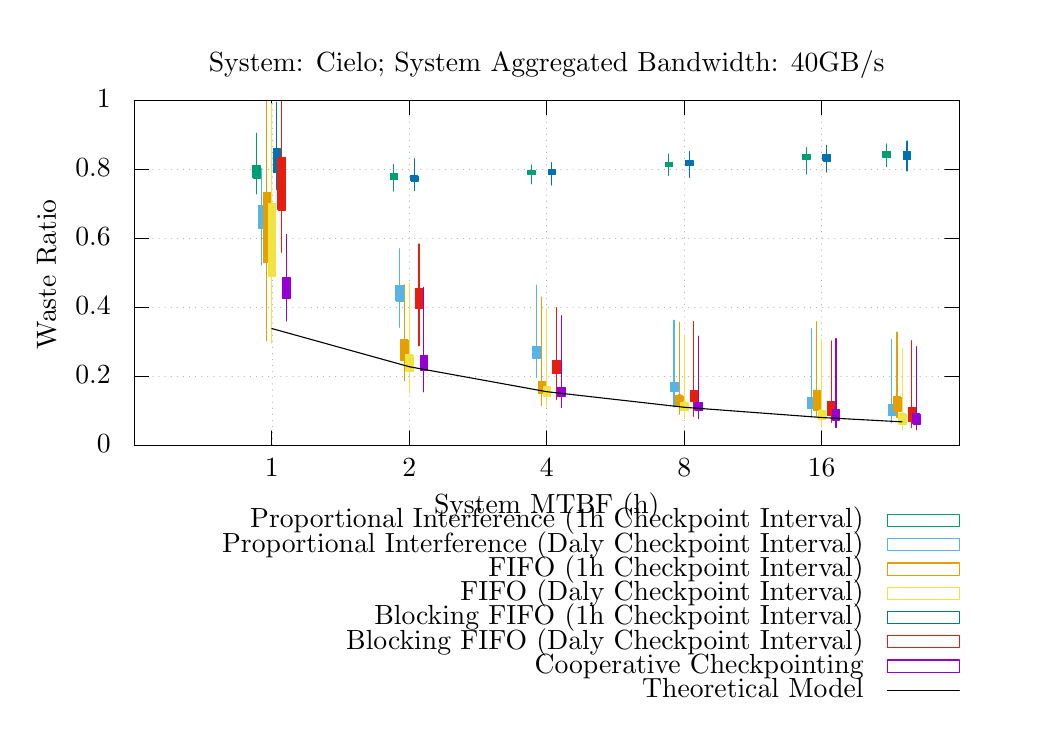
\begin{tikzpicture}[gnuplot]
%% generated with GNUPLOT 5.0p6 (Lua 5.3; terminal rev. 99, script rev. 100)
%% Wed Oct 18 12:29:40 2017
\path (0.000,0.000) rectangle (12.500,8.750);
\gpcolor{color=gp lt color axes}
\gpsetlinetype{gp lt axes}
\gpsetdashtype{gp dt axes}
\gpsetlinewidth{0.50}
\draw[gp path] (1.320,3.449)--(11.793,3.449);
\gpcolor{color=gp lt color border}
\gpsetlinetype{gp lt border}
\gpsetdashtype{gp dt solid}
\gpsetlinewidth{1.00}
\draw[gp path] (1.320,3.449)--(1.500,3.449);
\draw[gp path] (11.793,3.449)--(11.613,3.449);
\node[gp node right] at (1.136,3.449) {$0$};
\gpcolor{color=gp lt color axes}
\gpsetlinetype{gp lt axes}
\gpsetdashtype{gp dt axes}
\gpsetlinewidth{0.50}
\draw[gp path] (1.320,4.324)--(11.793,4.324);
\gpcolor{color=gp lt color border}
\gpsetlinetype{gp lt border}
\gpsetdashtype{gp dt solid}
\gpsetlinewidth{1.00}
\draw[gp path] (1.320,4.324)--(1.500,4.324);
\draw[gp path] (11.793,4.324)--(11.613,4.324);
\node[gp node right] at (1.136,4.324) {$0.2$};
\gpcolor{color=gp lt color axes}
\gpsetlinetype{gp lt axes}
\gpsetdashtype{gp dt axes}
\gpsetlinewidth{0.50}
\draw[gp path] (1.320,5.199)--(11.793,5.199);
\gpcolor{color=gp lt color border}
\gpsetlinetype{gp lt border}
\gpsetdashtype{gp dt solid}
\gpsetlinewidth{1.00}
\draw[gp path] (1.320,5.199)--(1.500,5.199);
\draw[gp path] (11.793,5.199)--(11.613,5.199);
\node[gp node right] at (1.136,5.199) {$0.4$};
\gpcolor{color=gp lt color axes}
\gpsetlinetype{gp lt axes}
\gpsetdashtype{gp dt axes}
\gpsetlinewidth{0.50}
\draw[gp path] (1.320,6.075)--(11.793,6.075);
\gpcolor{color=gp lt color border}
\gpsetlinetype{gp lt border}
\gpsetdashtype{gp dt solid}
\gpsetlinewidth{1.00}
\draw[gp path] (1.320,6.075)--(1.500,6.075);
\draw[gp path] (11.793,6.075)--(11.613,6.075);
\node[gp node right] at (1.136,6.075) {$0.6$};
\gpcolor{color=gp lt color axes}
\gpsetlinetype{gp lt axes}
\gpsetdashtype{gp dt axes}
\gpsetlinewidth{0.50}
\draw[gp path] (1.320,6.950)--(11.793,6.950);
\gpcolor{color=gp lt color border}
\gpsetlinetype{gp lt border}
\gpsetdashtype{gp dt solid}
\gpsetlinewidth{1.00}
\draw[gp path] (1.320,6.950)--(1.500,6.950);
\draw[gp path] (11.793,6.950)--(11.613,6.950);
\node[gp node right] at (1.136,6.950) {$0.8$};
\gpcolor{color=gp lt color axes}
\gpsetlinetype{gp lt axes}
\gpsetdashtype{gp dt axes}
\gpsetlinewidth{0.50}
\draw[gp path] (1.320,7.825)--(11.793,7.825);
\gpcolor{color=gp lt color border}
\gpsetlinetype{gp lt border}
\gpsetdashtype{gp dt solid}
\gpsetlinewidth{1.00}
\draw[gp path] (1.320,7.825)--(1.500,7.825);
\draw[gp path] (11.793,7.825)--(11.613,7.825);
\node[gp node right] at (1.136,7.825) {$1$};
\gpcolor{color=gp lt color axes}
\gpsetlinetype{gp lt axes}
\gpsetdashtype{gp dt axes}
\gpsetlinewidth{0.50}
\draw[gp path] (3.065,3.449)--(3.065,7.825);
\gpcolor{color=gp lt color border}
\gpsetlinetype{gp lt border}
\gpsetdashtype{gp dt solid}
\gpsetlinewidth{1.00}
\draw[gp path] (3.065,3.449)--(3.065,3.629);
\draw[gp path] (3.065,7.825)--(3.065,7.645);
\node[gp node center] at (3.065,3.141) {1};
\gpcolor{color=gp lt color axes}
\gpsetlinetype{gp lt axes}
\gpsetdashtype{gp dt axes}
\gpsetlinewidth{0.50}
\draw[gp path] (4.811,3.449)--(4.811,7.825);
\gpcolor{color=gp lt color border}
\gpsetlinetype{gp lt border}
\gpsetdashtype{gp dt solid}
\gpsetlinewidth{1.00}
\draw[gp path] (4.811,3.449)--(4.811,3.629);
\draw[gp path] (4.811,7.825)--(4.811,7.645);
\node[gp node center] at (4.811,3.141) {2};
\gpcolor{color=gp lt color axes}
\gpsetlinetype{gp lt axes}
\gpsetdashtype{gp dt axes}
\gpsetlinewidth{0.50}
\draw[gp path] (6.556,3.449)--(6.556,7.825);
\gpcolor{color=gp lt color border}
\gpsetlinetype{gp lt border}
\gpsetdashtype{gp dt solid}
\gpsetlinewidth{1.00}
\draw[gp path] (6.556,3.449)--(6.556,3.629);
\draw[gp path] (6.556,7.825)--(6.556,7.645);
\node[gp node center] at (6.556,3.141) {4};
\gpcolor{color=gp lt color axes}
\gpsetlinetype{gp lt axes}
\gpsetdashtype{gp dt axes}
\gpsetlinewidth{0.50}
\draw[gp path] (8.302,3.449)--(8.302,7.825);
\gpcolor{color=gp lt color border}
\gpsetlinetype{gp lt border}
\gpsetdashtype{gp dt solid}
\gpsetlinewidth{1.00}
\draw[gp path] (8.302,3.449)--(8.302,3.629);
\draw[gp path] (8.302,7.825)--(8.302,7.645);
\node[gp node center] at (8.302,3.141) {8};
\gpcolor{color=gp lt color axes}
\gpsetlinetype{gp lt axes}
\gpsetdashtype{gp dt axes}
\gpsetlinewidth{0.50}
\draw[gp path] (10.048,3.449)--(10.048,7.825);
\gpcolor{color=gp lt color border}
\gpsetlinetype{gp lt border}
\gpsetdashtype{gp dt solid}
\gpsetlinewidth{1.00}
\draw[gp path] (10.048,3.449)--(10.048,3.629);
\draw[gp path] (10.048,7.825)--(10.048,7.645);
\node[gp node center] at (10.048,3.141) {16};
\draw[gp path] (1.320,7.825)--(1.320,3.449)--(11.793,3.449)--(11.793,7.825)--cycle;
\node[gp node center,rotate=-270] at (0.246,5.637) {Waste Ratio};
\node[gp node center] at (6.556,2.679) {System MTBF (h)};
\node[gp node center] at (6.556,8.287) {System: Cielo; System Aggregated Bandwidth: 40GB/s};
\node[gp node right] at (10.698,2.490) {Proportional Interference (1h Checkpoint Interval)};
\gpcolor{rgb color={0.000,0.620,0.451}}
\draw[gp path] (10.882,2.413)--(11.798,2.413)--(11.798,2.567)--(10.882,2.567)--cycle;
\gpfill{rgb color={0.000,0.620,0.451}} (2.824,6.846)--(2.914,6.846)--(2.914,7.004)--(2.824,7.004)--cycle;
\draw[gp path] (2.869,6.639)--(2.869,6.846);
\draw[gp path] (2.869,7.004)--(2.869,7.409);
\draw[gp path] (2.824,7.004)--(2.914,7.004)--(2.914,6.846)--(2.824,6.846)--cycle;
\gpfill{rgb color={0.000,0.620,0.451}} (4.570,6.825)--(4.660,6.825)--(4.660,6.894)--(4.570,6.894)--cycle;
\draw[gp path] (4.615,6.675)--(4.615,6.825);
\draw[gp path] (4.615,6.894)--(4.615,7.013);
\draw[gp path] (4.570,6.894)--(4.660,6.894)--(4.660,6.825)--(4.570,6.825)--cycle;
\gpfill{rgb color={0.000,0.620,0.451}} (6.315,6.889)--(6.405,6.889)--(6.405,6.937)--(6.315,6.937)--cycle;
\draw[gp path] (6.360,6.767)--(6.360,6.889);
\draw[gp path] (6.360,6.937)--(6.360,7.007);
\draw[gp path] (6.315,6.937)--(6.405,6.937)--(6.405,6.889)--(6.315,6.889)--cycle;
\gpfill{rgb color={0.000,0.620,0.451}} (8.061,6.990)--(8.151,6.990)--(8.151,7.037)--(8.061,7.037)--cycle;
\draw[gp path] (8.106,6.874)--(8.106,6.990);
\draw[gp path] (8.106,7.037)--(8.106,7.145);
\draw[gp path] (8.061,7.037)--(8.151,7.037)--(8.151,6.990)--(8.061,6.990)--cycle;
\gpfill{rgb color={0.000,0.620,0.451}} (9.806,7.079)--(9.896,7.079)--(9.896,7.140)--(9.806,7.140)--cycle;
\draw[gp path] (9.851,6.891)--(9.851,7.079);
\draw[gp path] (9.851,7.140)--(9.851,7.226);
\draw[gp path] (9.806,7.140)--(9.896,7.140)--(9.896,7.079)--(9.806,7.079)--cycle;
\gpfill{rgb color={0.000,0.620,0.451}} (10.827,7.106)--(10.917,7.106)--(10.917,7.177)--(10.827,7.177)--cycle;
\draw[gp path] (10.872,6.987)--(10.872,7.106);
\draw[gp path] (10.872,7.177)--(10.872,7.273);
\draw[gp path] (10.827,7.177)--(10.917,7.177)--(10.917,7.106)--(10.827,7.106)--cycle;
\gpsetpointsize{0.80}
\gppoint{gp mark 2}{(2.869,6.931)}
\gppoint{gp mark 2}{(4.615,6.859)}
\gppoint{gp mark 2}{(6.360,6.911)}
\gppoint{gp mark 2}{(8.106,7.012)}
\gppoint{gp mark 2}{(9.851,7.106)}
\gppoint{gp mark 2}{(10.872,7.141)}
\gpcolor{color=gp lt color border}
\node[gp node right] at (10.698,2.182) {Proportional Interference (Daly Checkpoint Interval)};
\gpcolor{rgb color={0.337,0.706,0.914}}
\draw[gp path] (10.882,2.105)--(11.798,2.105)--(11.798,2.259)--(10.882,2.259)--cycle;
\gpfill{rgb color={0.337,0.706,0.914}} (2.891,6.207)--(2.981,6.207)--(2.981,6.491)--(2.891,6.491)--cycle;
\draw[gp path] (2.936,5.733)--(2.936,6.207);
\draw[gp path] (2.936,6.491)--(2.936,6.962);
\draw[gp path] (2.891,6.491)--(2.981,6.491)--(2.981,6.207)--(2.891,6.207)--cycle;
\gpfill{rgb color={0.337,0.706,0.914}} (4.637,5.280)--(4.727,5.280)--(4.727,5.478)--(4.637,5.478)--cycle;
\draw[gp path] (4.682,4.945)--(4.682,5.280);
\draw[gp path] (4.682,5.478)--(4.682,5.943);
\draw[gp path] (4.637,5.478)--(4.727,5.478)--(4.727,5.280)--(4.637,5.280)--cycle;
\gpfill{rgb color={0.337,0.706,0.914}} (6.382,4.551)--(6.472,4.551)--(6.472,4.702)--(6.382,4.702)--cycle;
\draw[gp path] (6.427,4.305)--(6.427,4.551);
\draw[gp path] (6.427,4.702)--(6.427,5.480);
\draw[gp path] (6.382,4.702)--(6.472,4.702)--(6.472,4.551)--(6.382,4.551)--cycle;
\gpfill{rgb color={0.337,0.706,0.914}} (8.128,4.132)--(8.218,4.132)--(8.218,4.248)--(8.128,4.248)--cycle;
\draw[gp path] (8.173,3.934)--(8.173,4.132);
\draw[gp path] (8.173,4.248)--(8.173,5.034);
\draw[gp path] (8.128,4.248)--(8.218,4.248)--(8.218,4.132)--(8.128,4.132)--cycle;
\gpfill{rgb color={0.337,0.706,0.914}} (9.873,3.914)--(9.963,3.914)--(9.963,4.048)--(9.873,4.048)--cycle;
\draw[gp path] (9.918,3.807)--(9.918,3.914);
\draw[gp path] (9.918,4.048)--(9.918,4.927);
\draw[gp path] (9.873,4.048)--(9.963,4.048)--(9.963,3.914)--(9.873,3.914)--cycle;
\gpfill{rgb color={0.337,0.706,0.914}} (10.894,3.829)--(10.984,3.829)--(10.984,3.961)--(10.894,3.961)--cycle;
\draw[gp path] (10.939,3.731)--(10.939,3.829);
\draw[gp path] (10.939,3.961)--(10.939,4.791);
\draw[gp path] (10.894,3.961)--(10.984,3.961)--(10.984,3.829)--(10.894,3.829)--cycle;
\gppoint{gp mark 3}{(2.936,6.355)}
\gppoint{gp mark 3}{(4.682,5.380)}
\gppoint{gp mark 3}{(6.427,4.648)}
\gppoint{gp mark 3}{(8.173,4.222)}
\gppoint{gp mark 3}{(9.918,4.017)}
\gppoint{gp mark 3}{(10.939,3.939)}
\gpcolor{color=gp lt color border}
\node[gp node right] at (10.698,1.874) {FIFO (1h Checkpoint Interval)};
\gpcolor{rgb color={0.902,0.624,0.000}}
\draw[gp path] (10.882,1.797)--(11.798,1.797)--(11.798,1.951)--(10.882,1.951)--cycle;
\gpfill{rgb color={0.902,0.624,0.000}} (2.957,5.767)--(3.047,5.767)--(3.047,6.655)--(2.957,6.655)--cycle;
\draw[gp path] (3.002,4.772)--(3.002,5.767);
\draw[gp path] (3.002,6.655)--(3.002,7.825);
\draw[gp path] (2.957,6.655)--(3.047,6.655)--(3.047,5.767)--(2.957,5.767)--cycle;
\gpfill{rgb color={0.902,0.624,0.000}} (4.702,4.525)--(4.792,4.525)--(4.792,4.785)--(4.702,4.785)--cycle;
\draw[gp path] (4.747,4.264)--(4.747,4.525);
\draw[gp path] (4.747,4.785)--(4.747,5.485);
\draw[gp path] (4.702,4.785)--(4.792,4.785)--(4.792,4.525)--(4.702,4.525)--cycle;
\gpfill{rgb color={0.902,0.624,0.000}} (6.448,4.104)--(6.538,4.104)--(6.538,4.253)--(6.448,4.253)--cycle;
\draw[gp path] (6.493,3.950)--(6.493,4.104);
\draw[gp path] (6.493,4.253)--(6.493,5.329);
\draw[gp path] (6.448,4.253)--(6.538,4.253)--(6.538,4.104)--(6.448,4.104)--cycle;
\gpfill{rgb color={0.902,0.624,0.000}} (8.193,3.951)--(8.283,3.951)--(8.283,4.073)--(8.193,4.073)--cycle;
\draw[gp path] (8.238,3.839)--(8.238,3.951);
\draw[gp path] (8.238,4.073)--(8.238,5.011);
\draw[gp path] (8.193,4.073)--(8.283,4.073)--(8.283,3.951)--(8.193,3.951)--cycle;
\gpfill{rgb color={0.902,0.624,0.000}} (9.939,3.891)--(10.029,3.891)--(10.029,4.137)--(9.939,4.137)--cycle;
\draw[gp path] (9.984,3.813)--(9.984,3.891);
\draw[gp path] (9.984,4.137)--(9.984,5.015);
\draw[gp path] (9.939,4.137)--(10.029,4.137)--(10.029,3.891)--(9.939,3.891)--cycle;
\gpfill{rgb color={0.902,0.624,0.000}} (10.960,3.875)--(11.050,3.875)--(11.050,4.060)--(10.960,4.060)--cycle;
\draw[gp path] (11.005,3.799)--(11.005,3.875);
\draw[gp path] (11.005,4.060)--(11.005,4.883);
\draw[gp path] (10.960,4.060)--(11.050,4.060)--(11.050,3.875)--(10.960,3.875)--cycle;
\gppoint{gp mark 4}{(3.002,6.245)}
\gppoint{gp mark 4}{(4.747,4.675)}
\gppoint{gp mark 4}{(6.493,4.225)}
\gppoint{gp mark 4}{(8.238,4.080)}
\gppoint{gp mark 4}{(9.984,4.055)}
\gppoint{gp mark 4}{(11.005,4.015)}
\gpcolor{color=gp lt color border}
\node[gp node right] at (10.698,1.566) {FIFO (Daly Checkpoint Interval)};
\gpcolor{rgb color={0.941,0.894,0.259}}
\draw[gp path] (10.882,1.489)--(11.798,1.489)--(11.798,1.643)--(10.882,1.643)--cycle;
\gpfill{rgb color={0.941,0.894,0.259}} (3.020,5.597)--(3.110,5.597)--(3.110,6.515)--(3.020,6.515)--cycle;
\draw[gp path] (3.065,4.744)--(3.065,5.597);
\draw[gp path] (3.065,6.515)--(3.065,7.784);
\draw[gp path] (3.020,6.515)--(3.110,6.515)--(3.110,5.597)--(3.020,5.597)--cycle;
\gpfill{rgb color={0.941,0.894,0.259}} (4.766,4.392)--(4.856,4.392)--(4.856,4.598)--(4.766,4.598)--cycle;
\draw[gp path] (4.811,4.108)--(4.811,4.392);
\draw[gp path] (4.811,4.598)--(4.811,5.501);
\draw[gp path] (4.766,4.598)--(4.856,4.598)--(4.856,4.392)--(4.766,4.392)--cycle;
\gpfill{rgb color={0.941,0.894,0.259}} (6.511,4.067)--(6.601,4.067)--(6.601,4.190)--(6.511,4.190)--cycle;
\draw[gp path] (6.556,3.937)--(6.556,4.067);
\draw[gp path] (6.556,4.190)--(6.556,5.184);
\draw[gp path] (6.511,4.190)--(6.601,4.190)--(6.601,4.067)--(6.511,4.067)--cycle;
\gpfill{rgb color={0.941,0.894,0.259}} (8.257,3.893)--(8.347,3.893)--(8.347,3.989)--(8.257,3.989)--cycle;
\draw[gp path] (8.302,3.786)--(8.302,3.893);
\draw[gp path] (8.302,3.989)--(8.302,4.843);
\draw[gp path] (8.257,3.989)--(8.347,3.989)--(8.347,3.893)--(8.257,3.893)--cycle;
\gpfill{rgb color={0.941,0.894,0.259}} (10.003,3.775)--(10.093,3.775)--(10.093,3.893)--(10.003,3.893)--cycle;
\draw[gp path] (10.048,3.679)--(10.048,3.775);
\draw[gp path] (10.048,3.893)--(10.048,4.792);
\draw[gp path] (10.003,3.893)--(10.093,3.893)--(10.093,3.775)--(10.003,3.775)--cycle;
\gpfill{rgb color={0.941,0.894,0.259}} (11.024,3.720)--(11.114,3.720)--(11.114,3.845)--(11.024,3.845)--cycle;
\draw[gp path] (11.069,3.641)--(11.069,3.720);
\draw[gp path] (11.069,3.845)--(11.069,4.675);
\draw[gp path] (11.024,3.845)--(11.114,3.845)--(11.114,3.720)--(11.024,3.720)--cycle;
\gppoint{gp mark 5}{(3.065,6.077)}
\gppoint{gp mark 5}{(4.811,4.519)}
\gppoint{gp mark 5}{(6.556,4.174)}
\gppoint{gp mark 5}{(8.302,3.991)}
\gppoint{gp mark 5}{(10.048,3.885)}
\gppoint{gp mark 5}{(11.069,3.837)}
\gpcolor{color=gp lt color border}
\node[gp node right] at (10.698,1.258) {Blocking FIFO (1h Checkpoint Interval)};
\gpcolor{rgb color={0.000,0.447,0.698}}
\draw[gp path] (10.882,1.181)--(11.798,1.181)--(11.798,1.335)--(10.882,1.335)--cycle;
\gpfill{rgb color={0.000,0.447,0.698}} (3.083,6.912)--(3.173,6.912)--(3.173,7.210)--(3.083,7.210)--cycle;
\draw[gp path] (3.128,6.691)--(3.128,6.912);
\draw[gp path] (3.128,7.210)--(3.128,7.803);
\draw[gp path] (3.083,7.210)--(3.173,7.210)--(3.173,6.912)--(3.083,6.912)--cycle;
\gpfill{rgb color={0.000,0.447,0.698}} (4.828,6.807)--(4.918,6.807)--(4.918,6.870)--(4.828,6.870)--cycle;
\draw[gp path] (4.873,6.681)--(4.873,6.807);
\draw[gp path] (4.873,6.870)--(4.873,7.085);
\draw[gp path] (4.828,6.870)--(4.918,6.870)--(4.918,6.807)--(4.828,6.807)--cycle;
\gpfill{rgb color={0.000,0.447,0.698}} (6.574,6.896)--(6.664,6.896)--(6.664,6.943)--(6.574,6.943)--cycle;
\draw[gp path] (6.619,6.750)--(6.619,6.896);
\draw[gp path] (6.619,6.943)--(6.619,7.035);
\draw[gp path] (6.574,6.943)--(6.664,6.943)--(6.664,6.896)--(6.574,6.896)--cycle;
\gpfill{rgb color={0.000,0.447,0.698}} (8.319,7.000)--(8.409,7.000)--(8.409,7.067)--(8.319,7.067)--cycle;
\draw[gp path] (8.364,6.848)--(8.364,7.000);
\draw[gp path] (8.364,7.067)--(8.364,7.177);
\draw[gp path] (8.319,7.067)--(8.409,7.067)--(8.409,7.000)--(8.319,7.000)--cycle;
\gpfill{rgb color={0.000,0.447,0.698}} (10.065,7.060)--(10.155,7.060)--(10.155,7.138)--(10.065,7.138)--cycle;
\draw[gp path] (10.110,6.915)--(10.110,7.060);
\draw[gp path] (10.110,7.138)--(10.110,7.256);
\draw[gp path] (10.065,7.138)--(10.155,7.138)--(10.155,7.060)--(10.065,7.060)--cycle;
\gpfill{rgb color={0.000,0.447,0.698}} (11.086,7.079)--(11.176,7.079)--(11.176,7.174)--(11.086,7.174)--cycle;
\draw[gp path] (11.131,6.931)--(11.131,7.079);
\draw[gp path] (11.131,7.174)--(11.131,7.309);
\draw[gp path] (11.086,7.174)--(11.176,7.174)--(11.176,7.079)--(11.086,7.079)--cycle;
\gppoint{gp mark 6}{(3.128,7.093)}
\gppoint{gp mark 6}{(4.873,6.841)}
\gppoint{gp mark 6}{(6.619,6.919)}
\gppoint{gp mark 6}{(8.364,7.032)}
\gppoint{gp mark 6}{(10.110,7.099)}
\gppoint{gp mark 6}{(11.131,7.126)}
\gpcolor{color=gp lt color border}
\node[gp node right] at (10.698,0.950) {Blocking FIFO (Daly Checkpoint Interval)};
\gpcolor{rgb color={0.898,0.118,0.063}}
\draw[gp path] (10.882,0.873)--(11.798,0.873)--(11.798,1.027)--(10.882,1.027)--cycle;
\gpfill{rgb color={0.898,0.118,0.063}} (3.143,6.440)--(3.233,6.440)--(3.233,7.103)--(3.143,7.103)--cycle;
\draw[gp path] (3.188,5.896)--(3.188,6.440);
\draw[gp path] (3.188,7.103)--(3.188,7.824);
\draw[gp path] (3.143,7.103)--(3.233,7.103)--(3.233,6.440)--(3.143,6.440)--cycle;
\gpfill{rgb color={0.898,0.118,0.063}} (4.889,5.193)--(4.979,5.193)--(4.979,5.443)--(4.889,5.443)--cycle;
\draw[gp path] (4.934,4.709)--(4.934,5.193);
\draw[gp path] (4.934,5.443)--(4.934,6.003);
\draw[gp path] (4.889,5.443)--(4.979,5.443)--(4.979,5.193)--(4.889,5.193)--cycle;
\gpfill{rgb color={0.898,0.118,0.063}} (6.634,4.360)--(6.724,4.360)--(6.724,4.526)--(6.634,4.526)--cycle;
\draw[gp path] (6.679,4.025)--(6.679,4.360);
\draw[gp path] (6.679,4.526)--(6.679,5.193);
\draw[gp path] (6.634,4.526)--(6.724,4.526)--(6.724,4.360)--(6.634,4.360)--cycle;
\gpfill{rgb color={0.898,0.118,0.063}} (8.380,4.006)--(8.470,4.006)--(8.470,4.136)--(8.380,4.136)--cycle;
\draw[gp path] (8.425,3.814)--(8.425,4.006);
\draw[gp path] (8.425,4.136)--(8.425,5.018);
\draw[gp path] (8.380,4.136)--(8.470,4.136)--(8.470,4.006)--(8.380,4.006)--cycle;
\gpfill{rgb color={0.898,0.118,0.063}} (10.125,3.826)--(10.215,3.826)--(10.215,4.002)--(10.125,4.002)--cycle;
\draw[gp path] (10.170,3.739)--(10.170,3.826);
\draw[gp path] (10.170,4.002)--(10.170,4.772);
\draw[gp path] (10.125,4.002)--(10.215,4.002)--(10.215,3.826)--(10.125,3.826)--cycle;
\gpfill{rgb color={0.898,0.118,0.063}} (11.146,3.756)--(11.236,3.756)--(11.236,3.925)--(11.146,3.925)--cycle;
\draw[gp path] (11.191,3.671)--(11.191,3.756);
\draw[gp path] (11.191,3.925)--(11.191,4.774);
\draw[gp path] (11.146,3.925)--(11.236,3.925)--(11.236,3.756)--(11.146,3.756)--cycle;
\gppoint{gp mark 7}{(3.188,6.792)}
\gppoint{gp mark 7}{(4.934,5.324)}
\gppoint{gp mark 7}{(6.679,4.465)}
\gppoint{gp mark 7}{(8.425,4.114)}
\gppoint{gp mark 7}{(10.170,3.955)}
\gppoint{gp mark 7}{(11.191,3.885)}
\gpcolor{color=gp lt color border}
\node[gp node right] at (10.698,0.642) {Cooperative Checkpointing};
\gpcolor{rgb color={0.580,0.000,0.827}}
\draw[gp path] (10.882,0.565)--(11.798,0.565)--(11.798,0.719)--(10.882,0.719)--cycle;
\gpfill{rgb color={0.580,0.000,0.827}} (3.203,5.312)--(3.293,5.312)--(3.293,5.579)--(3.203,5.579)--cycle;
\draw[gp path] (3.248,5.025)--(3.248,5.312);
\draw[gp path] (3.248,5.579)--(3.248,6.125);
\draw[gp path] (3.203,5.579)--(3.293,5.579)--(3.293,5.312)--(3.203,5.312)--cycle;
\gpfill{rgb color={0.580,0.000,0.827}} (4.948,4.408)--(5.038,4.408)--(5.038,4.586)--(4.948,4.586)--cycle;
\draw[gp path] (4.993,4.124)--(4.993,4.408);
\draw[gp path] (4.993,4.586)--(4.993,5.452);
\draw[gp path] (4.948,4.586)--(5.038,4.586)--(5.038,4.408)--(4.948,4.408)--cycle;
\gpfill{rgb color={0.580,0.000,0.827}} (6.694,4.067)--(6.784,4.067)--(6.784,4.185)--(6.694,4.185)--cycle;
\draw[gp path] (6.739,3.925)--(6.739,4.067);
\draw[gp path] (6.739,4.185)--(6.739,5.093);
\draw[gp path] (6.694,4.185)--(6.784,4.185)--(6.784,4.067)--(6.694,4.067)--cycle;
\gpfill{rgb color={0.580,0.000,0.827}} (8.439,3.895)--(8.529,3.895)--(8.529,3.987)--(8.439,3.987)--cycle;
\draw[gp path] (8.484,3.785)--(8.484,3.895);
\draw[gp path] (8.484,3.987)--(8.484,4.832);
\draw[gp path] (8.439,3.987)--(8.529,3.987)--(8.529,3.895)--(8.439,3.895)--cycle;
\gpfill{rgb color={0.580,0.000,0.827}} (10.185,3.773)--(10.275,3.773)--(10.275,3.897)--(10.185,3.897)--cycle;
\draw[gp path] (10.230,3.672)--(10.230,3.773);
\draw[gp path] (10.230,3.897)--(10.230,4.801);
\draw[gp path] (10.185,3.897)--(10.275,3.897)--(10.275,3.773)--(10.185,3.773)--cycle;
\gpfill{rgb color={0.580,0.000,0.827}} (11.206,3.722)--(11.296,3.722)--(11.296,3.846)--(11.206,3.846)--cycle;
\draw[gp path] (11.251,3.642)--(11.251,3.722);
\draw[gp path] (11.251,3.846)--(11.251,4.698);
\draw[gp path] (11.206,3.846)--(11.296,3.846)--(11.296,3.722)--(11.206,3.722)--cycle;
\gppoint{gp mark 1}{(3.248,5.451)}
\gppoint{gp mark 1}{(4.993,4.518)}
\gppoint{gp mark 1}{(6.739,4.173)}
\gppoint{gp mark 1}{(8.484,3.992)}
\gppoint{gp mark 1}{(10.230,3.884)}
\gppoint{gp mark 1}{(11.251,3.836)}
\gpcolor{color=gp lt color border}
\node[gp node right] at (10.698,0.334) {Theoretical Model};
\gpcolor{rgb color={0.000,0.000,0.000}}
\draw[gp path] (10.882,0.334)--(11.798,0.334);
\draw[gp path] (3.065,4.929)--(4.811,4.444)--(6.556,4.127)--(8.302,3.929)--(10.048,3.799)%
  --(11.069,3.744);
\gpcolor{color=gp lt color border}
\draw[gp path] (1.320,7.825)--(1.320,3.449)--(11.793,3.449)--(11.793,7.825)--cycle;
%% coordinates of the plot area
\gpdefrectangularnode{gp plot 1}{\pgfpoint{1.320cm}{3.449cm}}{\pgfpoint{11.793cm}{7.825cm}}
\end{tikzpicture}
%% gnuplot variables
}
  \end{center}
  \caption{Waste ratio as a function of the system MTBF for the
    seven I/O and Checkpointing scheduling strategies, and the LANL workload on
    Cielo. \label{fig:cielo-40gbs}}
\end{figure}

\paragraph{The Impact of System Reliability}
Second, we explore the performance of each approach under low bandwidth (and
thus high risk of interference). A scenarios with such low bandwidth is not
unrealistic, as mentioned in Luu et al~\cite{Luu:2015:Multiplatform} practical
bandwidth can be consideraly lower than the theoretical.
Figure~\ref{fig:cielo-40gbs} represents the waste ratio on Cielo, assuming the
aggregated filesystem bandwidth of the system was 40GB/s. We vary the node MTBF
$\muind$ from 2 years (1h of system MTBF) to 50 years (24h of system MTBF) in
order to evaluate the impact of this parameter. Similarly to
Figure~\ref{fig:cielo-1hmtbf}, we observe three classes of behavior: \propfixed
and \bfifofixed exhibit a waste ratio that remains constant around 80\% for all
values of the MTBF. These approaches are critically dependent on the filesystem
bandwidth, and a lower frequency of failures does not significantly improve
their performance. The I/O subsystem is saturated, and the applications spends
most of their time waiting for it.
%
\propdaly and \bfifodaly, see poor efficiency for small MTBF values, but
steadily improve to come close to the theoretical bound for higher MTBF values.
Last, \fifodaly, \fifofixed, and \cooperative quickly reach the theoretical
model performance, even with a challenging MTBF (4 years of node MTBF; or 2h of
system MTBF).

For all the strategies that integrate the Daly checkpointing period
optimization, increasing the MTBF reduces the amount of I/O required
and thus relieves the pressure of a constrained bandwidth. All
strategies that schedule the bandwidth are successful at increasing the
efficiency close to the theoretical model.
%
Similarly to the previous result, \fifofixed, despite its fixed checkpoint
interval is capable of reaching a performance comparable to the Daly-based
strategies that reduce the number of checkpoints. The quick improvement of the
\fifofixed approach can be explained by a combination of 2 factors. Foremost,
the non-blocking aspect of the checkpoint, provide the I/O subsystem with enough
flexibility to order the checkpoint without imposing additional wait. Delayed
checkpoints only translate in additional waste if that application itself is
subject to failure. Additionally, for small MTBFs, the more frequent restarts of
other jobs despite the fact that they delay the checkpointing operation do not
introduce additional waste.

%% HT + GB: we wanted to say the same thing but in a more clear setting
% Surprisingly so in the case of \fifofixed, with its fixed checkpoint
% interval, which is capable of reaching a performance
% comparable to the strategies that reduce the number of
% checkpoints. At 2h of system MTBF (4 years of node MTBF), the
% supplementary I/O from restarting processes competes with the high
% fixed checkpoint frequency for scarce I/O resources, resulting in
% significant wastage. However, at 8h of system MTBF (16 years of node
% MTBF), the number of restarts is greatly reduced and the non blocking
% checkpointing approach is sufficient to even the I/O load efficiently.

\subsection{Evaluating a Prospective System}

\begin{figure}
  \begin{center}
    \resizebox{\linewidth}{!}{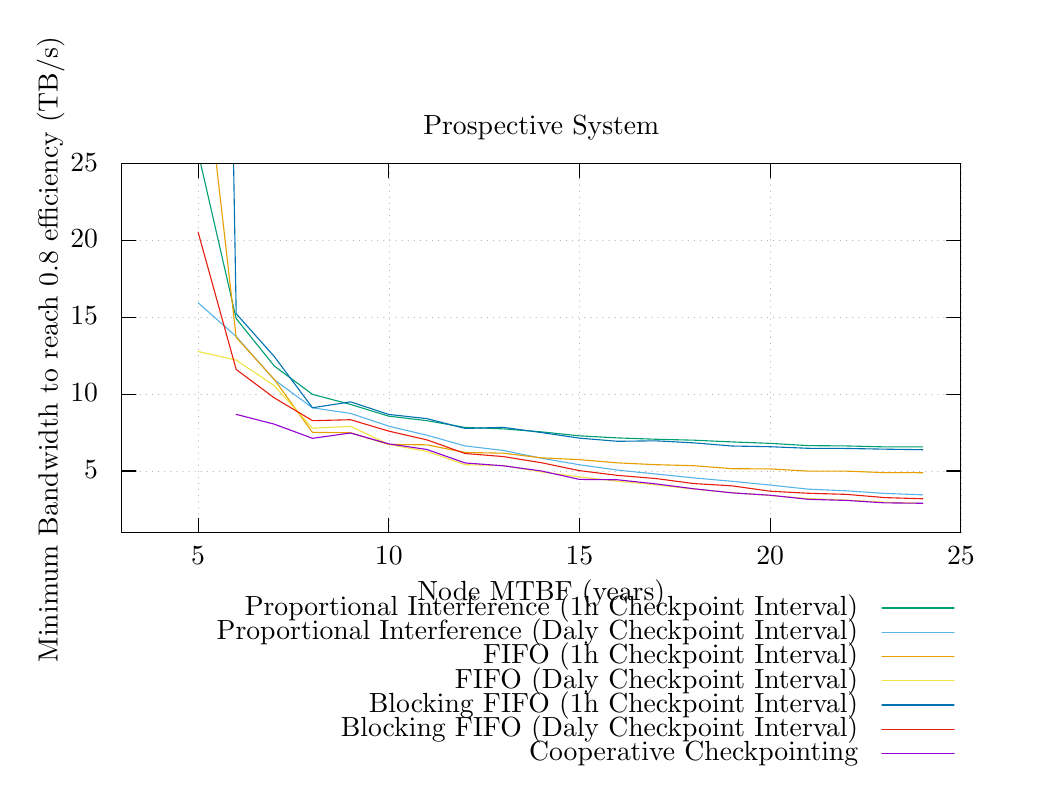
\begin{tikzpicture}[gnuplot]
%% generated with GNUPLOT 5.0p6 (Lua 5.3; terminal rev. 99, script rev. 100)
%% Wed Oct 18 12:29:10 2017
\path (0.000,0.000) rectangle (12.500,8.750);
\gpcolor{color=gp lt color axes}
\gpsetlinetype{gp lt axes}
\gpsetdashtype{gp dt axes}
\gpsetlinewidth{0.50}
\draw[gp path] (1.136,3.922)--(11.793,3.922);
\gpcolor{color=gp lt color border}
\gpsetlinetype{gp lt border}
\gpsetdashtype{gp dt solid}
\gpsetlinewidth{1.00}
\draw[gp path] (1.136,3.922)--(1.316,3.922);
\draw[gp path] (11.793,3.922)--(11.613,3.922);
\node[gp node right] at (0.952,3.922) {$5$};
\gpcolor{color=gp lt color axes}
\gpsetlinetype{gp lt axes}
\gpsetdashtype{gp dt axes}
\gpsetlinewidth{0.50}
\draw[gp path] (1.136,4.898)--(11.793,4.898);
\gpcolor{color=gp lt color border}
\gpsetlinetype{gp lt border}
\gpsetdashtype{gp dt solid}
\gpsetlinewidth{1.00}
\draw[gp path] (1.136,4.898)--(1.316,4.898);
\draw[gp path] (11.793,4.898)--(11.613,4.898);
\node[gp node right] at (0.952,4.898) {$10$};
\gpcolor{color=gp lt color axes}
\gpsetlinetype{gp lt axes}
\gpsetdashtype{gp dt axes}
\gpsetlinewidth{0.50}
\draw[gp path] (1.136,5.873)--(11.793,5.873);
\gpcolor{color=gp lt color border}
\gpsetlinetype{gp lt border}
\gpsetdashtype{gp dt solid}
\gpsetlinewidth{1.00}
\draw[gp path] (1.136,5.873)--(1.316,5.873);
\draw[gp path] (11.793,5.873)--(11.613,5.873);
\node[gp node right] at (0.952,5.873) {$15$};
\gpcolor{color=gp lt color axes}
\gpsetlinetype{gp lt axes}
\gpsetdashtype{gp dt axes}
\gpsetlinewidth{0.50}
\draw[gp path] (1.136,6.849)--(11.793,6.849);
\gpcolor{color=gp lt color border}
\gpsetlinetype{gp lt border}
\gpsetdashtype{gp dt solid}
\gpsetlinewidth{1.00}
\draw[gp path] (1.136,6.849)--(1.316,6.849);
\draw[gp path] (11.793,6.849)--(11.613,6.849);
\node[gp node right] at (0.952,6.849) {$20$};
\gpcolor{color=gp lt color axes}
\gpsetlinetype{gp lt axes}
\gpsetdashtype{gp dt axes}
\gpsetlinewidth{0.50}
\draw[gp path] (1.136,7.825)--(11.793,7.825);
\gpcolor{color=gp lt color border}
\gpsetlinetype{gp lt border}
\gpsetdashtype{gp dt solid}
\gpsetlinewidth{1.00}
\draw[gp path] (1.136,7.825)--(1.316,7.825);
\draw[gp path] (11.793,7.825)--(11.613,7.825);
\node[gp node right] at (0.952,7.825) {$25$};
\gpcolor{color=gp lt color axes}
\gpsetlinetype{gp lt axes}
\gpsetdashtype{gp dt axes}
\gpsetlinewidth{0.50}
\draw[gp path] (2.105,3.141)--(2.105,7.825);
\gpcolor{color=gp lt color border}
\gpsetlinetype{gp lt border}
\gpsetdashtype{gp dt solid}
\gpsetlinewidth{1.00}
\draw[gp path] (2.105,3.141)--(2.105,3.321);
\draw[gp path] (2.105,7.825)--(2.105,7.645);
\node[gp node center] at (2.105,2.833) {$5$};
\gpcolor{color=gp lt color axes}
\gpsetlinetype{gp lt axes}
\gpsetdashtype{gp dt axes}
\gpsetlinewidth{0.50}
\draw[gp path] (4.527,3.141)--(4.527,7.825);
\gpcolor{color=gp lt color border}
\gpsetlinetype{gp lt border}
\gpsetdashtype{gp dt solid}
\gpsetlinewidth{1.00}
\draw[gp path] (4.527,3.141)--(4.527,3.321);
\draw[gp path] (4.527,7.825)--(4.527,7.645);
\node[gp node center] at (4.527,2.833) {$10$};
\gpcolor{color=gp lt color axes}
\gpsetlinetype{gp lt axes}
\gpsetdashtype{gp dt axes}
\gpsetlinewidth{0.50}
\draw[gp path] (6.949,3.141)--(6.949,7.825);
\gpcolor{color=gp lt color border}
\gpsetlinetype{gp lt border}
\gpsetdashtype{gp dt solid}
\gpsetlinewidth{1.00}
\draw[gp path] (6.949,3.141)--(6.949,3.321);
\draw[gp path] (6.949,7.825)--(6.949,7.645);
\node[gp node center] at (6.949,2.833) {$15$};
\gpcolor{color=gp lt color axes}
\gpsetlinetype{gp lt axes}
\gpsetdashtype{gp dt axes}
\gpsetlinewidth{0.50}
\draw[gp path] (9.371,3.141)--(9.371,7.825);
\gpcolor{color=gp lt color border}
\gpsetlinetype{gp lt border}
\gpsetdashtype{gp dt solid}
\gpsetlinewidth{1.00}
\draw[gp path] (9.371,3.141)--(9.371,3.321);
\draw[gp path] (9.371,7.825)--(9.371,7.645);
\node[gp node center] at (9.371,2.833) {$20$};
\gpcolor{color=gp lt color axes}
\gpsetlinetype{gp lt axes}
\gpsetdashtype{gp dt axes}
\gpsetlinewidth{0.50}
\draw[gp path] (11.793,3.141)--(11.793,7.825);
\gpcolor{color=gp lt color border}
\gpsetlinetype{gp lt border}
\gpsetdashtype{gp dt solid}
\gpsetlinewidth{1.00}
\draw[gp path] (11.793,3.141)--(11.793,3.321);
\draw[gp path] (11.793,7.825)--(11.793,7.645);
\node[gp node center] at (11.793,2.833) {$25$};
\draw[gp path] (1.136,7.825)--(1.136,3.141)--(11.793,3.141)--(11.793,7.825)--cycle;
\node[gp node center,rotate=-270] at (0.246,5.483) {Minimum Bandwidth to reach 0.8 efficiency (TB/s)};
\node[gp node center] at (6.464,2.371) {Node MTBF (years)};
\node[gp node center] at (6.464,8.287) {Prospective System};
\node[gp node right] at (10.606,2.182) {Proportional Interference (1h Checkpoint Interval)};
\gpcolor{rgb color={0.000,0.620,0.451}}
\draw[gp path] (10.790,2.182)--(11.706,2.182);
\draw[gp path] (2.138,7.825)--(2.589,5.857)--(3.074,5.254)--(3.558,4.895)--(4.042,4.767)%
  --(4.527,4.618)--(5.011,4.561)--(5.496,4.475)--(5.980,4.457)--(6.465,4.419)--(6.949,4.368)%
  --(7.433,4.342)--(7.918,4.325)--(8.402,4.313)--(8.887,4.291)--(9.371,4.273)--(9.855,4.244)%
  --(10.340,4.240)--(10.824,4.228)--(11.309,4.228);
\gpcolor{color=gp lt color border}
\node[gp node right] at (10.606,1.874) {Proportional Interference (Daly Checkpoint Interval)};
\gpcolor{rgb color={0.337,0.706,0.914}}
\draw[gp path] (10.790,1.874)--(11.706,1.874);
\draw[gp path] (2.105,6.059)--(2.589,5.630)--(3.074,5.080)--(3.558,4.724)--(4.042,4.653)%
  --(4.527,4.491)--(5.011,4.376)--(5.496,4.240)--(5.980,4.183)--(6.465,4.084)--(6.949,4.001)%
  --(7.433,3.933)--(7.918,3.884)--(8.402,3.834)--(8.887,3.791)--(9.371,3.743)--(9.855,3.691)%
  --(10.340,3.670)--(10.824,3.637)--(11.309,3.619);
\gpcolor{color=gp lt color border}
\node[gp node right] at (10.606,1.566) {FIFO (1h Checkpoint Interval)};
\gpcolor{rgb color={0.902,0.624,0.000}}
\draw[gp path] (10.790,1.566)--(11.706,1.566);
\draw[gp path] (2.337,7.825)--(2.589,5.619)--(3.074,5.083)--(3.558,4.412)--(4.042,4.407)%
  --(4.527,4.259)--(5.011,4.254)--(5.496,4.157)--(5.980,4.148)--(6.465,4.089)--(6.949,4.066)%
  --(7.433,4.025)--(7.918,4.002)--(8.402,3.989)--(8.887,3.951)--(9.371,3.948)--(9.855,3.920)%
  --(10.340,3.920)--(10.824,3.901)--(11.309,3.900);
\gpcolor{color=gp lt color border}
\node[gp node right] at (10.606,1.258) {FIFO (Daly Checkpoint Interval)};
\gpcolor{rgb color={0.941,0.894,0.259}}
\draw[gp path] (10.790,1.258)--(11.706,1.258);
\draw[gp path] (2.105,5.440)--(2.589,5.330)--(3.074,5.005)--(3.558,4.466)--(4.042,4.489)%
  --(4.527,4.260)--(5.011,4.170)--(5.496,4.002)--(5.980,3.991)--(6.465,3.910)--(6.949,3.847)%
  --(7.433,3.792)--(7.918,3.747)--(8.402,3.691)--(8.887,3.646)--(9.371,3.610)--(9.855,3.572)%
  --(10.340,3.553)--(10.824,3.526)--(11.309,3.510);
\gpcolor{color=gp lt color border}
\node[gp node right] at (10.606,0.950) {Blocking FIFO (1h Checkpoint Interval)};
\gpcolor{rgb color={0.000,0.447,0.698}}
\draw[gp path] (10.790,0.950)--(11.706,0.950);
\draw[gp path] (2.556,7.825)--(2.589,5.919)--(3.074,5.374)--(3.558,4.725)--(4.042,4.800)%
  --(4.527,4.640)--(5.011,4.587)--(5.496,4.462)--(5.980,4.476)--(6.465,4.410)--(6.949,4.339)%
  --(7.433,4.299)--(7.918,4.305)--(8.402,4.279)--(8.887,4.239)--(9.371,4.230)--(9.855,4.210)%
  --(10.340,4.208)--(10.824,4.199)--(11.309,4.192);
\gpcolor{color=gp lt color border}
\node[gp node right] at (10.606,0.642) {Blocking FIFO (Daly Checkpoint Interval)};
\gpcolor{rgb color={0.898,0.118,0.063}}
\draw[gp path] (10.790,0.642)--(11.706,0.642);
\draw[gp path] (2.105,6.956)--(2.589,5.211)--(3.074,4.850)--(3.558,4.561)--(4.042,4.573)%
  --(4.527,4.428)--(5.011,4.317)--(5.496,4.144)--(5.980,4.105)--(6.465,4.027)--(6.949,3.926)%
  --(7.433,3.866)--(7.918,3.826)--(8.402,3.762)--(8.887,3.733)--(9.371,3.665)--(9.855,3.639)%
  --(10.340,3.625)--(10.824,3.584)--(11.309,3.569);
\gpcolor{color=gp lt color border}
\node[gp node right] at (10.606,0.334) {Cooperative Checkpointing};
\gpcolor{rgb color={0.580,0.000,0.827}}
\draw[gp path] (10.790,0.334)--(11.706,0.334);
\draw[gp path] (2.589,4.641)--(3.074,4.516)--(3.558,4.337)--(4.042,4.404)--(4.527,4.266)%
  --(5.011,4.195)--(5.496,4.024)--(5.980,3.988)--(6.465,3.922)--(6.949,3.815)--(7.433,3.810)%
  --(7.918,3.758)--(8.402,3.696)--(8.887,3.644)--(9.371,3.614)--(9.855,3.562)--(10.340,3.548)%
  --(10.824,3.517)--(11.309,3.512);
\gpcolor{color=gp lt color border}
\draw[gp path] (1.136,7.825)--(1.136,3.141)--(11.793,3.141)--(11.793,7.825)--cycle;
%% coordinates of the plot area
\gpdefrectangularnode{gp plot 1}{\pgfpoint{1.136cm}{3.141cm}}{\pgfpoint{11.793cm}{7.825cm}}
\end{tikzpicture}
%% gnuplot variables
}
  \end{center}
  \caption{Minimum aggregated filesystem bandwidth to reach 80\%
    efficiency with the different approaches on the prospective
    future system.\label{fig:prosp}}
\end{figure}

In order to understand the impact of the I/O contention on future platforms, we
use our simulator to explore a prospective system and assess the impact of I/O
and checkpoint scheduling when the problem size and the machine size will
increase. We consider a future system with 7PB of main memory and 50,000 compute
nodes (Aurora\footnote{\url{https://aurora.alcf.anl.gov/}}). Based on the APEX
workflow report, we extrapolate the increase in problem size expected for the
application classes considered above, and project these applications on the
prospective system.  We simulate the workload of Table~\ref{table:lanl}, scaling
the problem size proportionally to the change in machine memory size. The waste
is computed, as previously, by dividing the amount of resource used for
checkpoints and lost due to failures by the amount of resource used in a
fault-free and resilience-free run with the same initial conditions.
%
We consider different values for the system MTBF; and for each strategy, we
find the required aggregated practical bandwidth necessary to provide a
sustained 80\% efficiency of the system.
%
Figure~\ref{fig:prosp} shows the impact of the MTBF and of the
different strategies on this system.

When the failures are frequent (under 10 years of node MTBF), the most critical
element is to reduce the I/O pressure: all strategies that use a fixed and
frequent checkpoint interval require a much higher system bandwidth to reach the
target efficiency.  In this case, strategies that combine an optimal
checkpointing period with I/O and checkpoint scheduling (\cooperative and
\fifodaly) perform similarly, consistently better than all other approaches.
These 2 approaches exhibit a strong resilience to failures, with a bandwidth
requirement that only increases by a factor 3 between a very unstable system (at
less than 1h of system MTBF), and a stable one (at 8h of system MTBF). On the
contrary, the other strategies are much more dependent upon the frequency of
failures, with the \propfixed strategy requiring up to 50 times the bandwidth of
\cooperative to reach the same efficiency under these MTBF conditions.

When failures are not an endemic
event, \ie as soon as the node MTBF is at least 15 years
(corresponding to a system MTBF of 2.6h), the hierarchy of different
approaches stabilizes: the two blocking strategies that rely on
frequent checkpoints (\propfixed and \bfifofixed) are the ones
requiring the highest bandwidth to maintain 80\%
efficiency. % 6.4TB/s at 24 years
\fifofixed, that uses a fixed checkpoint interval comes next, with a
requirement around three quarter of the one required by \propfixed and
\fifofixed. It benefits from the capacity to continue working when the
filesystem is not available to checkpoint, which is sufficient, when
failures are rare, to obtain a significant performance
gain. % 4.9TB/s at 24 years
Then the four strategies that use the Daly optimal checkpointing
period, alleviating significantly the I/O pressure, are the ones that
require the lowest bandwidth to reach 80\% of efficiency, at about
half the required bandwidth of the current
situation. %coop: 2.9 TB/s at 24 years


% !TEX root =  ipdps18.tex

\section{Related Work}\label{sec:related}
% Primary: Kurt

We first discuss research regarding checkpoint-induced I/O pressure, followed by
works that regard avoiding I/O interference.  These techniques are not necessarily
independent: generally, reducing I/O pressure will reduce the likelihood of
interference.  Therefore, we focus our I/O interference discussion to those
techniques which consider the global scheduling of checkpoints and/or application I/O
across a platform.

%\todo[inline]{kbf: I am unsure about this breakdown.  These two things do not
%seem independent; reducing pressure seems to al reduce interference ...}

\paragraph*{Checkpointing and I/O}

For a single application, the Young/Daly formula~\cite{young74,daly04} gives the
optimal checkpointing period. This period minimizes platform waste, defined as the
fraction of job execution time that does not contribute to its progress.  The two
sources of waste are the time spent taking checkpoints (which motivates longer
checkpoint periods) and the time needed to recover and re-execute after each failure
(which motivates shorter checkpoint periods). The Young/Daly period achieves the
optimal trade-off between these sources to minimize the total waste. Arunagiri et
al.~\cite{Arunagiri2010} studied longer, sub-optimal periods with the intent of
reducing I/O pressure and showed, both analytically and empircally using four real
platforms, that a decrease in the I/O requirement can be achieved with only a small
increase in waste.

\paragraph*{Reducing I/O Pressure}

There are two general strategies for reducing I/O pressure from a single application:
hiding or reducing checkpoint commit times without reducing checkpoint data volumes,
and reducing commit times by reducing checkpoint data volumes.  Strategies that
attempt to hide checkpoint times include Diskless~\cite{Plank98Diskless} and remote
checkpoint protocols~\cite{Cornwell11RemoteBLCR} which leverage the typically higher
available bandwidths of the network or other storage media like RAM in order to
mitigate the performance of slower storage media like spinning or solid-state
disks. Additionally, remotely stored checkpoints have the additional benefit of
allowing systems to survive non-transient node failures. Similarly, multi-level
checkpoint protocols like SCR~\cite{Moody10SCR,Vaidya95TwoLevel} attempt to hide
checkpoint commit times by writing checkpoints to RAM, flash storage, or local disk
on the compute nodes~\cite{Kougkas2017} in addition to the parallel file system
thereby improving checkpoint or general I/O bandwidth.  Finally, checkpoint-specific
file systems like PLFS~\cite{Bent09PLFS} leverage the I/O patterns and
characteristics specific to checkpoint data to optimize checkpoint data transfers
to/from parallel file systems and therefore reduce checkpoint commit times.

Strategies that attempt to reduce checkpoint sizes include \emph{memory
exclusion}, which leverage user-directives or other hints to exclude portions of
process address spaces from checkpoints~\cite{Plank99MemoryExclusion}.
Additionally, incremental checkpointing protocols reduce checkpoint volumes by
utilizing the OS's memory page protection facilities to detect and save only
pages that have been updated between consecutive
checkpoints~\cite{Bronevetsky09Compiler,
Chen97CLIP,Elnozahy92ConsistentCheckpointing,Li94ConcurrentCheckpointing,
Plank94Libckpt,Paun10IncrementalWeibull,Kiswany08stdchk}.  Similarly,
page-based hashing techniques can also be used to avoid checkpointing pages
that have been written to but whose content has not
changed~\cite{Ferreira11Libhashckpt}.  Finally, compression-based techniques
use standard compression algorithms to reduce checkpoint
volumes~\cite{Ibtesham12Compression} and can be used at the
compiler-level~\cite{Li90CATCH} or in-memory~\cite{Plank94ICKP}.  Related,
Plank et al. proposed \textit{differential compression} to reduce checkpoint
sizes for incremental checkpoints~\cite{Plank95CompressedDiff} and Tanzima et
al.  show that similarities amongst checkpoint data from different processes
can be exploited to compress and reduce checkpoint data
volumes~\cite{tanzima12mcrengine}.  Finally, Sasaki et al propose a lossy
compression method based on wavelet transform and vector quantization to the
checkpoints of a production climate application~\cite{sasaki2015}, while Ni et
al~\cite{Ni2014} study the trade-offs between the loss of precision, compression
ratio, and application correctness due to lossy compression.

\paragraph*{Avoiding I/O interference}

Most closely related to our work, a number of studies have considered the global
scheduling of checkpoints and other I/O across a platform to reduce overall
congestion, thereby increasing performance.  Aupy et al.~\cite{Aupy:2017:Periodic}
presented a decentralized I/O scheduling technique for minimizing the congestion due
to checkpoint interference by taking advantage of the observed periodic and
deterministic nature of HPC application checkpoints and I/O.  This technique allows
the job scheduler to pre-define each application’s I/O behavior for their entire
execution.  Similarly, a number of works have investigated the efficiency of online
schedulers for data intensive~\cite{Groot2013,Sim:2015:AnalyzeThis} and HPC workload
I/O~\cite{Dorier2015,Gainaru:2016:Scheduling,Zhou:2015:IOAware,Herbein2017}.
Finally, a number of works have investigated utilizing recorded system reliability
information~\cite{Oliner:2006:Cooperative} and the statistical properties of these
failures~\cite{Tiwari:2014:Lazy} to determine effective checkpoint intervals for the
portion of the system used by the workload.

\paragraph*{Summary}

We distinguish our work from these previous studies in a number of important ways.
First, unlike a number of the previous studies, our technique considers existing
non-CR application I/O. Additionally, our approach is agnostic to the I/O patterns of
the considered applications as long as they are known.  Also, we attempt to optimize
the efficiency of the entire platform, with the changing workloads and failures
running on that platform, rather than just considering one workload. Finally and most
importantly, this approach provides optimal checkpointing periods in environments
where I/O is highly constrained and Daly/Young's formula is less appropriate, a common
scenario on many leadership-class systems.

\section{Conclusion and Future Work}
\label{sec:conclusion}
% Primary: Aurélien

In this paper we presented a comprehensive model to capture interference
between multiple applications performing fault-tolerance related I/O
on a shared HPC system. We proved that ... We designed multiple algorithms
to schedule and order the checkpointing I/O workload, with the intent of
diminishing the average slowdown sustained by applications on the
platform induced by sharing the I/O subsystem, \ie improve the throughput
of the platform. We designed a event-based simulator that permits
executing typical HPC workloads on current and prospective systems.
With this simulator we have been able to offer guidances as to the
preferred heuristics for scheduling checkpoint workloads, and the
general I/O requirements for future HPC systems to sustain checkpointing.


\section*{Acknowledgement}

This material is based in part upon work supported by the National
Science Foundation under Grant Number 1564133, ``Toward Extreme Scale
Fault-Tolerance: Exploration Methods, Comparative Studies and Decision
Processes''.

\bibliographystyle{IEEEtran}
\bibliography{biblio}

%
%%%%%%%%%%%%%%%%%%%%%%%%%%%%%%%%%%%%%%%%%%%%%%%%%%%%%%%%%%%%%%%%%%%%%%%%
% FOLLOWUP TEXT IS OLDER AND MAY NEED MERGING OR DISCARDING
%%%%%%%%%%%%%%%%%%%%%%%%%%%%%%%%%%%%%%%%%%%%%%%%%%%%%%%%%%%%%%%%%%%%%%%%

\newpage
\appendix

\section{Exhaustive Results}

\begin{figure*}[t]
\noindent\begin{tabular}{C{.5\linewidth}C{.5\linewidth}}
For fixed values of the platform bandwidth & For fixed values of the platform MTBF \\
\includegraphics[width=\linewidth]{sim/figures/synthetic-040gbs-waste-celio.pdf} & \includegraphics[width=\linewidth]{sim/figures/synthetic-01hMTBF-waste-celio.pdf} \\
\includegraphics[width=\linewidth]{sim/figures/synthetic-080gbs-waste-celio.pdf} & \includegraphics[width=\linewidth]{sim/figures/synthetic-02hMTBF-waste-celio.pdf} \\
\includegraphics[width=\linewidth]{sim/figures/synthetic-120gbs-waste-celio.pdf} & \includegraphics[width=\linewidth]{sim/figures/synthetic-08hMTBF-waste-celio.pdf} \\
\includegraphics[width=\linewidth]{sim/figures/synthetic-160gbs-waste-celio.pdf} & \includegraphics[width=\linewidth]{sim/figures/synthetic-24hMTBF-waste-celio.pdf} \\
\end{tabular}
\caption{Celio, Waste}
\end{figure*}

\clearpage

\begin{figure*}[t]
\noindent\begin{tabular}{C{.02\linewidth}C{.49\linewidth}C{.49\linewidth}}
     ~    &  Checkpoint Period: 1H & Checkpoint Period: Daly \\
\rotatebox[origin=c]{90}{Overall Waste} & \includegraphics[width=\linewidth]{sim/figures/1hMTBF-1hckpt-waste-celio.pdf} & \includegraphics[width=\linewidth]{sim/figures/1hMTBF-dalyckpt-waste-celio.pdf} \\
\rotatebox[origin=c]{90}{Checkpointing} & \includegraphics[width=\linewidth]{sim/figures/1hMTBF-1hckpt-ckpt-celio.pdf} & \includegraphics[width=\linewidth]{sim/figures/1hMTBF-dalyckpt-ckpt-celio.pdf} \\
\rotatebox[origin=c]{90}{Usefull Work} & \includegraphics[width=\linewidth]{sim/figures/1hMTBF-1hckpt-work-celio.pdf} & \includegraphics[width=\linewidth]{sim/figures/1hMTBF-dalyckpt-work-celio.pdf} \\
\rotatebox[origin=c]{90}{Usefull I/O} & \includegraphics[width=\linewidth]{sim/figures/1hMTBF-1hckpt-io-celio.pdf} & \includegraphics[width=\linewidth]{sim/figures/1hMTBF-dalyckpt-io-celio.pdf}
\end{tabular}
\caption{Celio, Fixed MTBF: 1H}
\end{figure*}

\clearpage

\begin{figure*}[t]
\noindent\begin{tabular}{C{.02\linewidth}C{.49\linewidth}C{.49\linewidth}}
     ~    &  Checkpoint Period: 1H & Checkpoint Period: Daly \\
\rotatebox[origin=c]{90}{Overall Waste} & \includegraphics[width=\linewidth]{sim/figures/40gbs-1hckpt-waste-celio.pdf} & \includegraphics[width=\linewidth]{sim/figures/40gbs-dalyckpt-waste-celio.pdf} \\
\rotatebox[origin=c]{90}{Checkpointing} & \includegraphics[width=\linewidth]{sim/figures/40gbs-1hckpt-ckpt-celio.pdf} & \includegraphics[width=\linewidth]{sim/figures/40gbs-dalyckpt-ckpt-celio.pdf} \\
\rotatebox[origin=c]{90}{Usefull Work} & \includegraphics[width=\linewidth]{sim/figures/40gbs-1hckpt-work-celio.pdf} & \includegraphics[width=\linewidth]{sim/figures/40gbs-dalyckpt-work-celio.pdf} \\
\rotatebox[origin=c]{90}{Usefull I/O} & \includegraphics[width=\linewidth]{sim/figures/40gbs-1hckpt-io-celio.pdf} & \includegraphics[width=\linewidth]{sim/figures/40gbs-dalyckpt-io-celio.pdf}
\end{tabular}
\caption{Celio, Fixed Bandwidth: 40GB/s}
\end{figure*}

\clearpage


\section{Older text}



\subsection{Checkpointing and I/O}

For a single application, the optimal checkpointing period is given by the Young/Daly
formula~\cite{young74,daly04}. This period minimizes the platform waste, defined as
the fraction of the
execution time that does not contribute to the progress of the application (the
time \emph{wasted}).  There are two sources of waste, the time spent taking checkpoints
(which calls for longer checkpoint periods),
and the time needed to recover and re-execute after each failure
(which calls for shorter checkpoint periods),
The Young/Daly
period achieves the optimal trade-off between both sources to minimize the
total waste.
However, this optimal period may put too much pressure
on the I/O system. It is possible to use a longer, sub-optimal, period that would incur
less pressure and still lead to a reasonable waste. S. Arunagiri et al.~\cite{Arunagiri2009} have studied such trade-offs and they have shown, both analytically and instantiating the model with four real-life platforms,
that a great decrease in I/O requirement can be achieved  at the price of a small increase of the waste.

\subsection{I/O interference}


\section{Execution Model}
\label{sec.model}


\section{Optimal Checkpointing Period under I/O constraint}
\label{sec.optimal}

The waste of an application is the ratio of time that the application spends doing
resilience operations by the time that it does useful work. The time
spent doing resilience operations include the time spend during each period to checkpoint, and in case of failure, the time to rollback to the previous checkpoint, and the time to recompute lost work. We assume
that the rollback time is equivalent to the checkpoint time, and we
can define the waste $\wasteapp{i}$ of an application of class
$\app{i}$ as follows (\cite{springer-monograph}):

\begin{equation}
\wasteapp{i} = \wastefct{i}{\ckpt{i}} = \frac{\ckpt{i}}{\period{i}} +
\frac{\nbnodes{i}}{\mtbfplat}(\frac{\period{i}}{2} + \ckpt{i})
\label{eq.wasteAi}
\end{equation}

Let $\wasteplat$ be the waste of the platform. We define this as the
weighted arithmetic mean of the $\wasteapp{i}$ for all applications
(where each application is weighted by the number of computing nodes
it uses):

\begin{equation}
\wasteplat = \sum_i \frac{\nbapp{i} \nbnodes{i}}{\nbnodesplat} \wasteapp{i}
\label{eq.waste}
\end{equation}

In the absence of I/O constraints, the checkpointing period can be minimized
for each application independently. Indeed, the optimal period for an application
of class $\app{i}$ is obtained by minimizing $\wasteapp{i}$ in Equation~\eqref{eq.wasteAi}.
Differentiating and solving
$$\frac{\delta \wasteapp{i}}{\delta \period{i}} = - \frac{\ckpt{i}}{\period{i}^{2}} + \frac{\nbnodes{i}}{2 \mtbfplat} = 0$$
we readily derive that
\begin{equation}
\period{i} = \sqrt{2 \frac{\mtbfplat}{\nbnodes{i}} \ckpt{i}} = \sqrt{2 \mu_{i} \ckpt{i}}
\label{eq.daly}
\end{equation}
where $\mu_{i}$ is the MTBF of  class $\app{i}$ applications, which is the Young/Daly formula~\cite{young74,daly04}.
\todo[inline]{So they were right! We might want to define what $\period{i}$
  stands for before the reader reaches this point and can figure it by
  itself}

However, I/O constraints impose the use of sub-optimal periods. If each application
of  class $\app{i}$ checkpoints in time $\ckpt{i}$ during its period $\period{i}$ (hence without any contention), it uses the I/O device during a fraction $\frac{\ckpt{i}}{\period{i}}$ of the time.
The total usage fraction of the  I/O device is $\sum_{i} \frac{\nbapp{i} \ckpt{i}}{\period{i}}$
and cannot exceed $1$. Therefore, we have to solve the following optimization problem: find
the set of values $\period{i}$ that minimize $\wasteplat$ in Equation~\eqref{eq.waste} subject to the I/O constraint:

\begin{equation}
\sum_{i} \frac{\nbapp{i} \ckpt{i}}{\period{i}} \leq 1
\label{eq.IOconstraint}
\end{equation}

Note that Equation~\eqref{eq.IOconstraint} is a necessary condition, but is may not be sufficient:
even though the total I/O bandwidth is not exceeded, meaning there is enough capacity to take all the checkpoints at the given periods, we still need to orchestrate these checkpoints so that there is no contention. We come back to this point below.

The optimization problem writes: minimize $\wasteplat = \sum_i \frac{\nbapp{i} \nbnodes{i}}{\nbnodesplat}  \left( \frac{\ckpt{i}}{\period{i}} +
\frac{\nbnodes{i}}{\mtbfplat}(\frac{\period{i}}{2} + \ckpt{i}) \right)$
subject to $\ioconstraint = \sum_{i} \frac{\nbapp{i} \ckpt{i}}{\period{i}} \leq 1$.
Using the Karush-Kuhn-Tucker condition, we know that there exists a nonnegative constant
$\lambda$
such that
$$- \frac{\delta \wasteplat}{\delta \period{i}} = \lambda \frac{\delta\ioconstraint }{\delta \period{i}}$$
for all $i$. We derive that
$$\frac{\nbapp{i} \nbnodes{i} \ckpt{i}}{\nbnodesplat \period{i}^{2}} -    \frac{\nbapp{i} \nbnodes{i}^{2}}{2 \mtbfplat \nbnodesplat} = - \lambda \frac{\nbapp{i} \ckpt{i}}{\period{i}^{2}}
$$
for all $i$. This leads to:
 \begin{equation}
\period{i} = \sqrt{\frac{2 \mtbfplat  \nbnodesplat}{\nbnodes{i}^{2}} \left(\frac{\nbnodes{i}}{\nbnodesplat} +\lambda \right) \ckpt{i}}
  \label{eq.KKT}
\end{equation}
for all $i$. Note that when $\lambda=0$, Equation~\eqref{eq.KKT} reduces to Equation~\eqref{eq.daly}. Because of the I/O constraint in Equation~\eqref{eq.IOconstraint},
we will choose for $\lambda$ the minimum value such that Equation~\eqref{eq.IOconstraint}
  is satisfied. This will lead to periods $P_{i}$ larger than the optimal value of Equation~\eqref{eq.daly}.
  Note that there is no closed-form expression for the minimum value of $\lambda$,
  it has to be found numerically.
   Altogether, we state our main result:

   \begin{theorem}
  In the presence of I/O constraints, the optimal values of the checkpointing periods are given
  by Equation~\eqref{eq.KKT}, where $\lambda$ is the smallest nonnegative value such that
  Equation~\ref{eq.IOconstraint} holds.
\end{theorem}

\section{Optimal Cooperative Checkpointing Strategy}
\label{sec.strategy}

\subsection{With Burst Buffers}

We slightly change the machine model, and will consider that, in addition
to the global PFS, each node is provisioned with a local stage-in I/O
burst buffer. With burst buffers, $\ckpt{i}$ still represents the time it
takes to upload the checkpoint to the stable storage (the file system).
However, the availability of burst buffers permits a reduction in the
apparent time for the checkpoints as experienced by application idle
time. Note that under I/O constraints on the PFS, checkpoints may remain
in burst buffers (which is not a stable storage) until sufficient
PFS bandwidth is available.

Consider Algorithm~\ref{alg.withbb}: every $\period{i}$ time
units, each application of class $\app{i}$ takes a checkpoint and save
it onto the next free slot on the burst buffer; a global shared FIFO
queue transfers checkpoints from active slots in burst buffers onto
the parallel file system following the FIFO queue order.

\algblockdefx{Process}{EndProcess}[1]{\textbf{On Process} #1}{\textbf{End Process}}
\algnotext{EndProcess}
\algblockdefx{Every}{DoneEvery}[1]{\textbf{Every } #1}{\textbf{Done}}
\algnotext{DoneEvery}
\algblockdefx{When}{DoneWhen}[1]{\textbf{When } #1}{\textbf{Done}}
\algnotext{DoneWhen}
\algloopdefx{If}[1]{\textbf{If} #1 \textbf{then}}
\begin{algorithm}
\caption{Cooperative Checkpointing Algorithm with Burst Buffers}
\label{alg.withbb}
\begin{algorithmic}
\State \textbf{var} $transfer\_queue$, a FIFO initially empty
\Process{$p$, belonging to application $\application{i}{j}$ of class $\app{i}$}
   \State \textbf{var} $slots$ set of burst buffer files that can
   store a checkpoint
   \Every{$\period{i}$ time units}
           \State $slot  \gets $ oldest slot that is not being used for transfer
           \State Checkpoint application state into $slot$
           \If{$slot$ is marked done transferring}
                  \State Append $(p, slot)$ to $transfer\_queue$
    \DoneEvery
\EndProcess

\Process{$T$}
   \When{$transfer\_queue$ is not empty}
       \State Pop $slot$ from $transfer\_queue$
       \State Mark $slot$ as being transferred
       \State Transfer Checkpoint in $slot$ to File System
       \State Mark $slot$ as done transferring
   \DoneWhen
\EndProcess
\end{algorithmic}
\end{algorithm}

\begin{theorem}
  Algorithm~\ref{alg.withbb} ensures that all applications of class $\app{i}$
  checkpoint at most every $max(\sum_j\nbapp{j}*\ckpt{j}, \period{i})$
  time units, and requires only a burst buffer capable of storing 2
  checkpoints per process.
\end{theorem}

\begin{proof}
  \todo{This derives from $\sum_i \frac{\ckpt{i}}{\period{i}} \leq 1$,
    but should be done properly.}
\end{proof}

The theorem does provide a lower bound for the platform waste.\todo[inline]{the 2 storages holds only after the optimization, doesn't it? Or is it also a consequence of the above "proof" sketch?}
However, we have a FIFO system, and some applications may incur
a re-execution time larger than $P_{i}$. What is the worst case?
A first optimization is the following: when a checkpoint is taken
    by a given application, we check whether its previous checkpoint is
    still in the queue from the burst buffer to the file system. If yes, the new
checkpoint should \emph{replace} the old one, keeping the same position in the queue.
With this optimization, there is at most two checkpoints per application in the queue,
one being currently transferred and one waiting.
Then the worst case is to wait for the checkpoint of all the other applications.
Formally, the maximal re-execution time for application
$\application{i}{j}$ of class
$\app{i}$ is
$$\max(P_{i}, \sum_{k=1}^{\nbapps} n_{k}C_{k} - C_{i})$$

 \todo[inline]{Discussed at JLESC meeting: size of burst buffer can be
    bounded by 2 checkpoints easily, and it should be: if there are 3
    checkpoints in the burst buffer, then the first one might be being
    transferred, but this means that the 2nd is useless as we already
    reached the 3rd one. The 2nd should be discarded and its slot in
    the FIFO queue should be taken by the 3rd.}

  \todo[inline]{No clear what qualifies for burst buffers here, but
    currently the NVM bandwidth is (1) significantly lower than the
    network bandwidth, and (2) unidirectional. This might change in
    the future, but at least today it seems cheaper to use a
    buddy-checkpointing approach.}%


\subsection{Without Burst Buffers}

Without a local caching mechanism\footnote{Note that this case covers ``shared'' burst-buffers, where the
PFS contains an intermediate stage-in area (presumably with SSD drives, a much higher bandwidth, and possibly contention reduced to a subset of the nodes it serves, but provides for stable/persistent storage as soon as the data is committed to the shared burst-buffer.}, the times at which to take the checkpoint
must be scheduled to avoid any kind of checkpoint-checkpoint
interference (which can only waste resources, as all interfering
applications are slowed down while blocking on non-productive
operations). We consider here a centralized scheduler that decides at
any time what next application should checkpoint, and when.

The scheduler remembers when each application $\application{i}{j}$ of class
$\app{i}$ last initiated a checkpoint. We then define $\lastckpt{i}{j}$
as the time since the last checkpoint $\application{i}{j}$ started
(or since the start of $\application{i}{j}$ if none has been taken yet).
As soon as $\application{i}{j}$ has executed for $P_{i}$ time-units,
it is put in the checkpointing pool $\pool$ by the centralized scheduler. It
continues executing until it is selected from the pool to checkpoint.

Which application in the pool should be selected to checkpoint?
Assume that some previous checkpoint terminates at time $t$,
and let
$$\pool = \{ \application{i_{1}}{j_{1}}, \dots, \application{i_{k}}{j_{k}} \}$$
be the set of applications  in the pool at time $t$. All these applications are
candidate to checkpointing. At time $t$, each application $\application{i_{\ell}}{j_{\ell}} \in \pool$
has been executing for  $\lastckpt{i_{\ell}}{j_{\ell}}$ time-units.

If we select $\application{i_{\ell}}{j_{\ell}}$ to checkpoint (in time $C_{j_{\ell}}$),
and if there is a failure during that checkpoint, the time lost by every other application
$\application{i_{m}}{j_{m}} \in \pool$, $m \neq \ell$, is (in expectation) equal to
 $\lastckpt{i_m}{j_m} + \frac{C_{j_{\ell}}}{2}$.
We define the risk incurred by application
$\application{i_{m}}{j_{m}} \in \pool$, $m \neq \ell$
as its potential waste, which is the time lost divided by its MTBF $\frac{\mtbfplat}{\nbnodes{i}}$,
times the number $\nbnodes{i_m}$ processors enrolled by this application, i.e.
$$ \frac{\nbnodes{i_{m}}}{\mtbfplat}  (\lastckpt{i_m}{j_m} + \frac{C_{j_{\ell}}}{2})
\times \nbnodes{i_m} $$
Altogether, selecting $\application{i_{\ell}}{j_{\ell}}$ to checkpoint leads to a total risk
$$\risk(\application{i_{\ell}}{j_{\ell}}) = \sum_{1 \leq m \leq k, m \neq \ell} \frac{\nbnodes{i_{m}}^{2}}{\mtbfplat}  \times (\lastckpt{i_m}{j_m} + \frac{C_{j_{\ell}}}{2})$$
  for all applications that stayed in the pool.

We greedily choose the application in the pool that minimizes the risk:
$$\application{i_{\ell}}{j_{\ell}} = Argmin_{\application{i_m}{j_m} \in \pool} \risk(\application{i_m}{j_m})$$

%At the end of each checkpointing, the scheduler selects
%$\application{i}{j}$ such that
%$$
%\left\{
%\begin{array}{l}
%\nbnodes{i}(\frac{\wastefct{i}{\lastckpt{i}{j}}}{\wastefct{i}{\period{i}}}) \textrm{ if }\lastckpt{i}{j}\geq\period{i}\\
%0\textrm{ if }\lastckpt{i}{j}<\period{i}\\
%\end{array}\right.$$
%is maximal and strictly superior to 0.

Two remarks:
\begin{itemize}
\item Because we put applications in the pool only after they have run for $P_{i}$ times-steps,
this greedy algorithm guarantees Young/Daly periods to every application
whenever there is non conflict to access I/O resources.
\item The final schedule is not periodic. Instead, it is constructed dynamically
after each checkpoint completion. Computing the actual waste can be achieved
through simulation, and compared to the lower bound of Section~\ref{sec.optimal}.
\end{itemize}


\end{document}
